\documentclass[11pt]{article}
\usepackage[margin=1in]{geometry}
\usepackage{amsmath,amssymb,amsthm}
\usepackage{booktabs}
\usepackage{array}
\usepackage{graphicx}
\usepackage{verbatim}
\usepackage[colorlinks=true,linkcolor=blue,citecolor=blue,urlcolor=blue]{hyperref}
\newcommand{\Q}{\mathbf{Q}}
\newcommand{\Z}{\mathbf{Z}}
\newcommand{\F}{\mathbf{F}}
\newcommand{\PP}{\mathbf{P}}
\newcommand{\NS}{\mathrm{NS}}
\newcommand{\X}{X}
\newtheorem*{theorem*}{Theorem}
\theoremstyle{remark}
\newtheorem*{remark*}{Remark}
\title{A genus 2 curve with 738 rational points}
\author{Andrew V. Sutherland}
\date{18 November 2026}
\begin{document}
\maketitle

\begin{abstract}
The genus 2 curve
\begin{align*}
C_{738}\colon\quad y^2 ={}& 743425x^6 - 16144220x^5 + 60026500x^4\\
& + 172162750x^3 + 40133975x^2 - 46160230x + 6838225
\end{align*}
has at least $738$ rational points, and its Jacobian is absolutely simple, of Mordell--Weil rank $21$ (the upper bound assumes GRH).
The previous record for a curve with simple Jacobian was $642$ (Elkies and Stoll, 2008), and the largest number published for any
curve of genus $2$ was $648$.  The curve is a line section of a double-plane model of the K3 surface of Picard number $20$ and
discriminant $-163$ whose branch sextic has three nodes.  It is found by a computation that is simple to state and to repeat.
Starting from the sextic model of the surface published by Elkies, construct sextics, in minimal coordinates, for $2381$ models of
the surface with at most three nodes; on each of them count the rational points of small height of the surface on every line of
height at most $400$; count rational points on the curves cut out by the lines with the most; and close the sets of points found
under the relation given by a cubic through four points.  The whole computation, from Elkies' sextic to the curves, takes about
an hour on a $16$-core computer.  It also finds a second new curve, with $654$ points, and the curve of Elkies and Stoll.  All $738$ points can be
regenerated from the five values $x=0,\pm\frac12,-\frac32,\frac13$ by repeatedly passing a cubic through four known points, a
certificate that runs in a web browser in under a minute.  The programs, their output, and certificates for the statements
made here accompany the note.
\end{abstract}

\section{Introduction}

For a curve of genus $g\ge 2$ over $\Q$ the number of rational points is finite, and Caporaso, Harris and
Mazur~\cite{CHM} showed that the Bombieri--Lang conjecture would imply a bound $B(g)$ depending only on $g$.  The
largest known number of points on a curve of genus $2$ therefore has some interest as a lower bound for $B(2)$.  The
history of the record is short: Keller and Kulesz~\cite{KK} found a curve with $588$ points in 1995, a curve with
twelve automorphisms and a split Jacobian, and at the end of 2008 Stoll, searching in families supplied by Elkies, found
\begin{align*}
C_{642}\colon\quad y^2 ={}& 82342800x^6 - 470135160x^5 + 52485681x^4\\
& + 2396040466x^3 + 567207969x^2 - 985905640x + 247747600
\end{align*}
with at least $642$ points~\cite{StollExp,StollAvg,StollRecord}.  It has no automorphism besides the hyperelliptic involution and
its Jacobian is absolutely simple: in that sense it is a generic curve.

Beating $642$ is one of the open problems that Epoch AI lists in its FrontierMath collection~\cite{Epoch}.  The problem puts no
condition on the Jacobian, and in 2026 it was solved by the model GPT-6 Astra with the curve
\[
y^2 = 98285087781x^6 - 1685253906933x^4 + 7793336764011x^2 + 83877673125,
\]
which has $648$ points.  Like the Keller--Kulesz curve it has twelve automorphisms and a split Jacobian ($648=12\cdot 54$).
Our aim was different: to beat $642$ with a generic curve.  The curve $C_{738}$ does that.  It also has more points
than the $648$-point curve, which was the largest number published for any curve of genus $2$.

\begin{theorem*}
The curve $C_{738}$ of the abstract has at least $738$ rational points: $369$ values of $x$, each with two values of $y$
(there are no rational Weierstrass points and no rational points at infinity).  All of them are obtained from the ten points
with $x\in\{0,\pm\frac12,-\frac32,\frac13\}$ by the four-point cubic closure of Section~\ref{sec:closure}.  The differences of
the known points generate a subgroup of rank $21$ of $J(\Q)$, where $J$ is the Jacobian; the group $J(\Q)$ is torsion-free;
the sextic has Galois group $S_6$, so $\mathrm{End}(J_{\overline\Q})=\Z$, $J$ is absolutely simple and the curve has no
automorphism besides the hyperelliptic involution.  Assuming GRH, the rank of $J(\Q)$ is exactly $21$.
\end{theorem*}

\noindent What is proved and what is not:
\begin{center}\small
\begin{tabular}{ll}
\toprule
statement & status\\
\midrule
at least $738$ rational points & proved; certificate in Section~\ref{sec:closure}\\
Galois group $S_6$, $\mathrm{End}(J_{\overline\Q})=\Z$, no torsion & proved (Section~\ref{sec:curve})\\
rank of $J(\Q)$ at least $21$ & proved (Section~\ref{sec:curve})\\
rank of $J(\Q)$ exactly $21$ & assumes GRH\\
exactly $738$ rational points & not proved; evidence in Section~\ref{sec:curve}\\
each of the $2381$ sextics searched is a model of $\X_{163}$ & proved (Section~\ref{sec:models})\\
the census of models is complete & not proved; evidence in Section~\ref{sec:surface}\\
the search finds every line section with many points & not claimed; Section~\ref{sec:results}\\
\bottomrule
\end{tabular}
\end{center}

\noindent\emph{The search in brief.}  One K3 surface has many models as a double cover of the plane, and each model carries its
own two-parameter family of genus $2$ curves, one for each line (Section~\ref{sec:strategy}).  The models are classes in a
lattice (Section~\ref{sec:surface}).  Starting from Elkies' sextic, and from nothing else, we construct sextics, in minimal
coordinates, for all the models with one or two nodes that we know of and for $2188$ of the $2192$ with three: $2381$ sextics
(Section~\ref{sec:models}).  On each sextic we list the rational points
of the surface of height at most $4000$ and count them on every line of height at most $400$; this number is the \emph{score} of
the line.  For the lines with a score of at least $40$ we count the rational points of height up to $10^5$ on the curve the line
cuts out (Section~\ref{sec:search}), and for the best of these curves we close the set of points under a relation that finds the
points of large height (Section~\ref{sec:closure}).  No step takes a curve as input, and nothing is tuned to a particular model.
The whole computation took $62$ minutes on a $16$-core machine, $7$ of them for the construction of the
models; its programs, its input and its output are in a public repository~\cite{Repo}.  Sixteen of the curves it finds have at least $600$ points,
and three have at least $642$: $C_{738}$, a second new curve with $654$ points, and $C_{642}$ itself
(Section~\ref{sec:results}).  Section~\ref{sec:curve} collects what is known about $C_{738}$, and Section~\ref{sec:files}
says where to find the files with which the statements of this note can be checked and the computation repeated.

\medskip\noindent\emph{What is taken from earlier work and what is new.}  The framework is that of Elkies and Stoll: line sections
of double-plane models of $\X_{163}$, with points forced by the curves on which the sextic is a square (Section~\ref{sec:strategy}),
a search of all lines up to a height bound, and Stoll's observation that further points can be found on cubics through known ones.
This note adds three things: a construction that produces sextics for $2381$ models from Elkies' one, where the search of 2008
used five; a score that ranks all the lines of a model at a cost of a fraction of a microsecond per line, the number of
rational points of small height of the surface on the line; and the four-point closure,
which finds the points of large height and, unlike the five-point test, enlarges the subgroup generated by the known points.

\begin{figure}[ht]
\centering
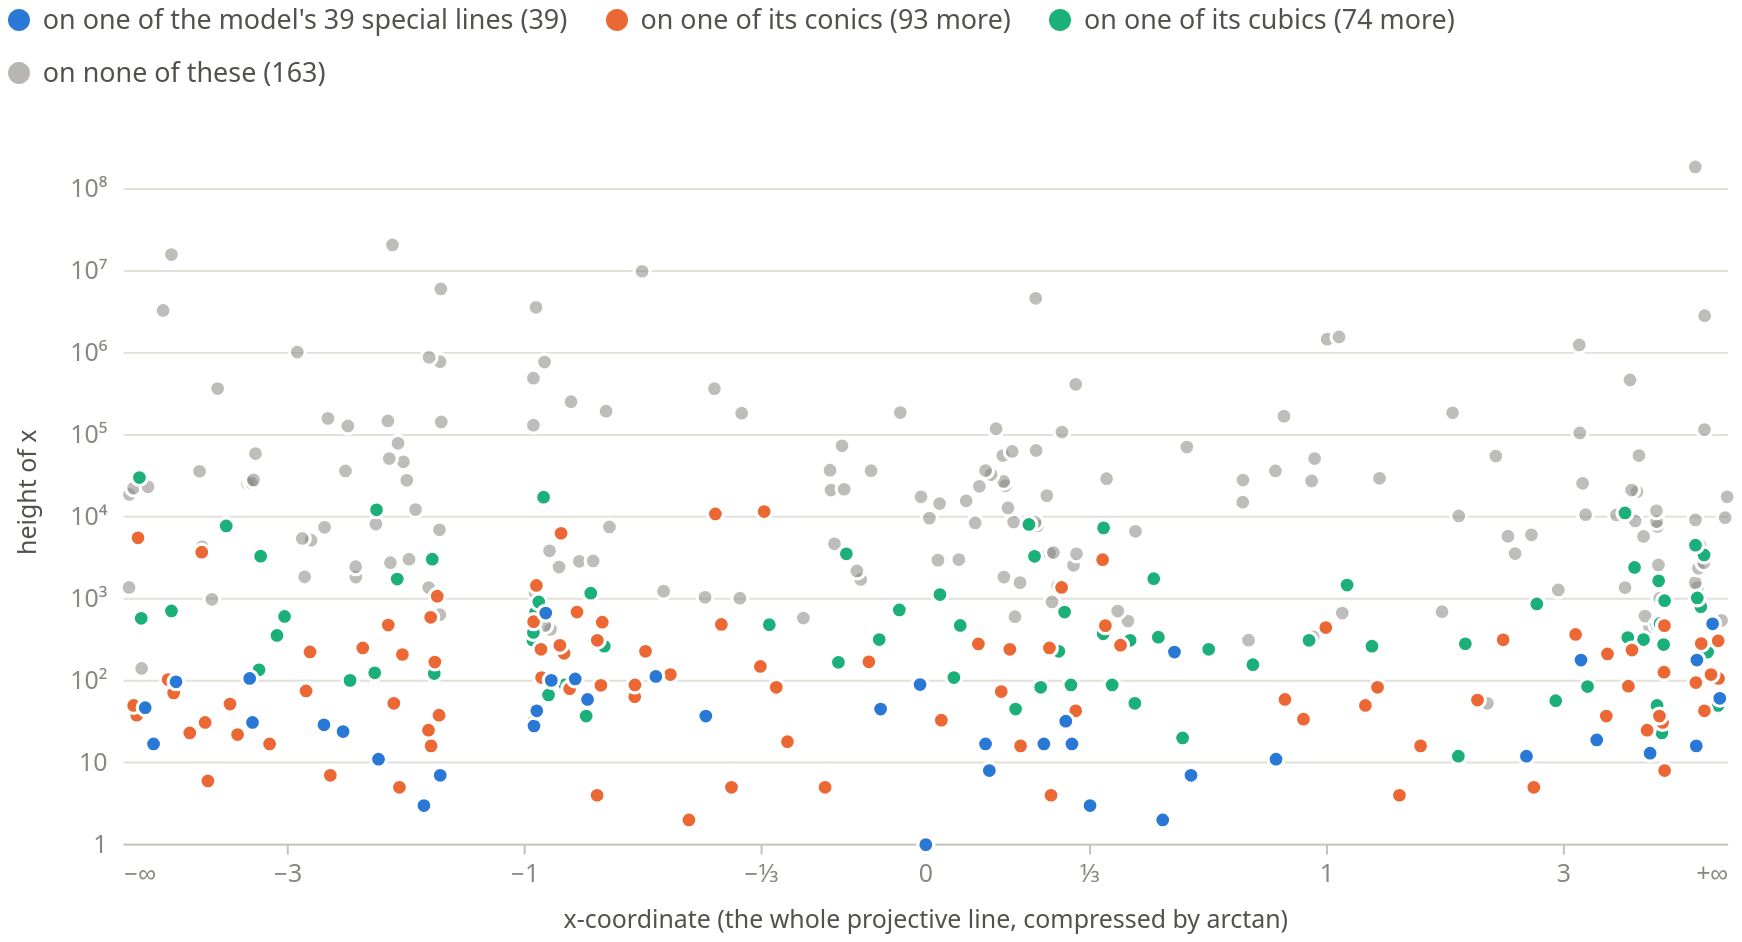
\includegraphics[width=\linewidth]{figs/xvalues.png}
\caption{Every rational point we know on $C_{738}$.  Each dot is one of the $369$ $x$-coordinates, placed by its position on the projective line and by its height; each stands for two points.  Blue: forced by one of the $39$ special lines of the model.  Orange: on one of its conics.  Green: on one of its cubics.  Gray: on none of these.  The colours record which tabulated curves of the model pass through a point, not how the point was found.  Height measures arithmetic size, not position: $x=1474359/1473364$ is close to $1$ and has height $1.5\times10^6$.}
\label{fig:xvalues}
\end{figure}

Throughout, the \emph{height} of $x=a/c$ in lowest terms is $\max(|a|,|c|)$, and the height of a line
$\lambda\colon ax_0+bx_1+cx_2=0$ with coprime integer coefficients is $\max(|a|,|b|,|c|)$; we write $\lambda=(a,b,c)$.

\section{The Elkies--Stoll strategy}\label{sec:strategy}

Let $\X$ be a K3 surface over $\Q$ and $D$ a divisor class with $D^2=2$ that is nef, with $|D|$ base-point free.  Then $|D|$
gives a map $\pi\colon\X\to\PP^2$ of degree $2$~\cite{SaintDonat}, branched along a sextic curve $B\colon S(x_0,x_1,x_2)=0$, and $\X$ is the
minimal resolution of the double plane
\[
w^2 = S(x_0,x_1,x_2).
\]
The smooth rational curves $E$ with $E\cdot D=0$ are contracted by $\pi$ to singular points of $B$ (a single such curve gives
a node).  The members of $|D|$ are the pullbacks of the lines: for a line $\lambda$ meeting $B$ in six distinct points,
\[
C_\lambda=\pi^{-1}(\lambda)\colon\quad y^2 = S|_\lambda
\]
is a curve of genus $2$, and the sextic on the right is just $S$ restricted to a parametrization of $\lambda$.  So every such
surface carries a two-parameter family of genus $2$ curves, indexed by the dual plane.

The point of the construction is that rational curves on $\X$ force rational points on the $C_\lambda$.  Suppose $\ell$
is a line on which $S$ restricts to a perfect square, $S|_\ell=G^2$.  Then $\pi^{-1}(\ell)$ splits into two rational curves
$w=\pm G$, and the point $\lambda\cap\ell$ lifts to \emph{two rational points} of $C_\lambda$, for every $\lambda\ne\ell$
(to one, if the point lies on $B$).  The restriction $S|_\ell$ is a constant times a square
when $\ell$ meets $B$ with even multiplicity at every point: when it is tangent to $B$ at three points (a \emph{tritangent}), or
passes through one or two nodes of $B$ and is tangent to $B$ wherever else it meets it (a \emph{node line}).  In general the
constant need not be a square in $\Q$.  On the surface used here it always is, because every divisor class is defined over $\Q$,
so both components of $\pi^{-1}(\ell)$ are.  A model with $N$ such lines therefore puts $2N$ rational points on
$C_\lambda$ whenever $\lambda$ meets the $N$ lines in $N$ distinct points, none of them on $B$.  Only the lines $\lambda$ through one
of finitely many points of the plane fail this (the points where two of the $N$ lines meet and the points they share with $B$),
and they get fewer.  We call these the \emph{forced points}, and say that the model has $2N$ of them.  The same mechanism works in higher degree.  If $c$ is a
conic with $S|_c$ a square, then $\lambda\cap c$ consists of two points, usually conjugate over a quadratic field; when
they happen to be rational they give, in general, four more rational points of $C_\lambda$.  Whether this happens is the condition that a
quadratic form in $(a,b,c)$, the discriminant of $\lambda$ restricted to $c$, is a square.  Cubics and curves of higher
degree behave in the same way.  A line $\lambda$ for which many of these independent conditions hold at once has a curve
$C_\lambda$ with many points.

\begin{figure}[ht]
\centering
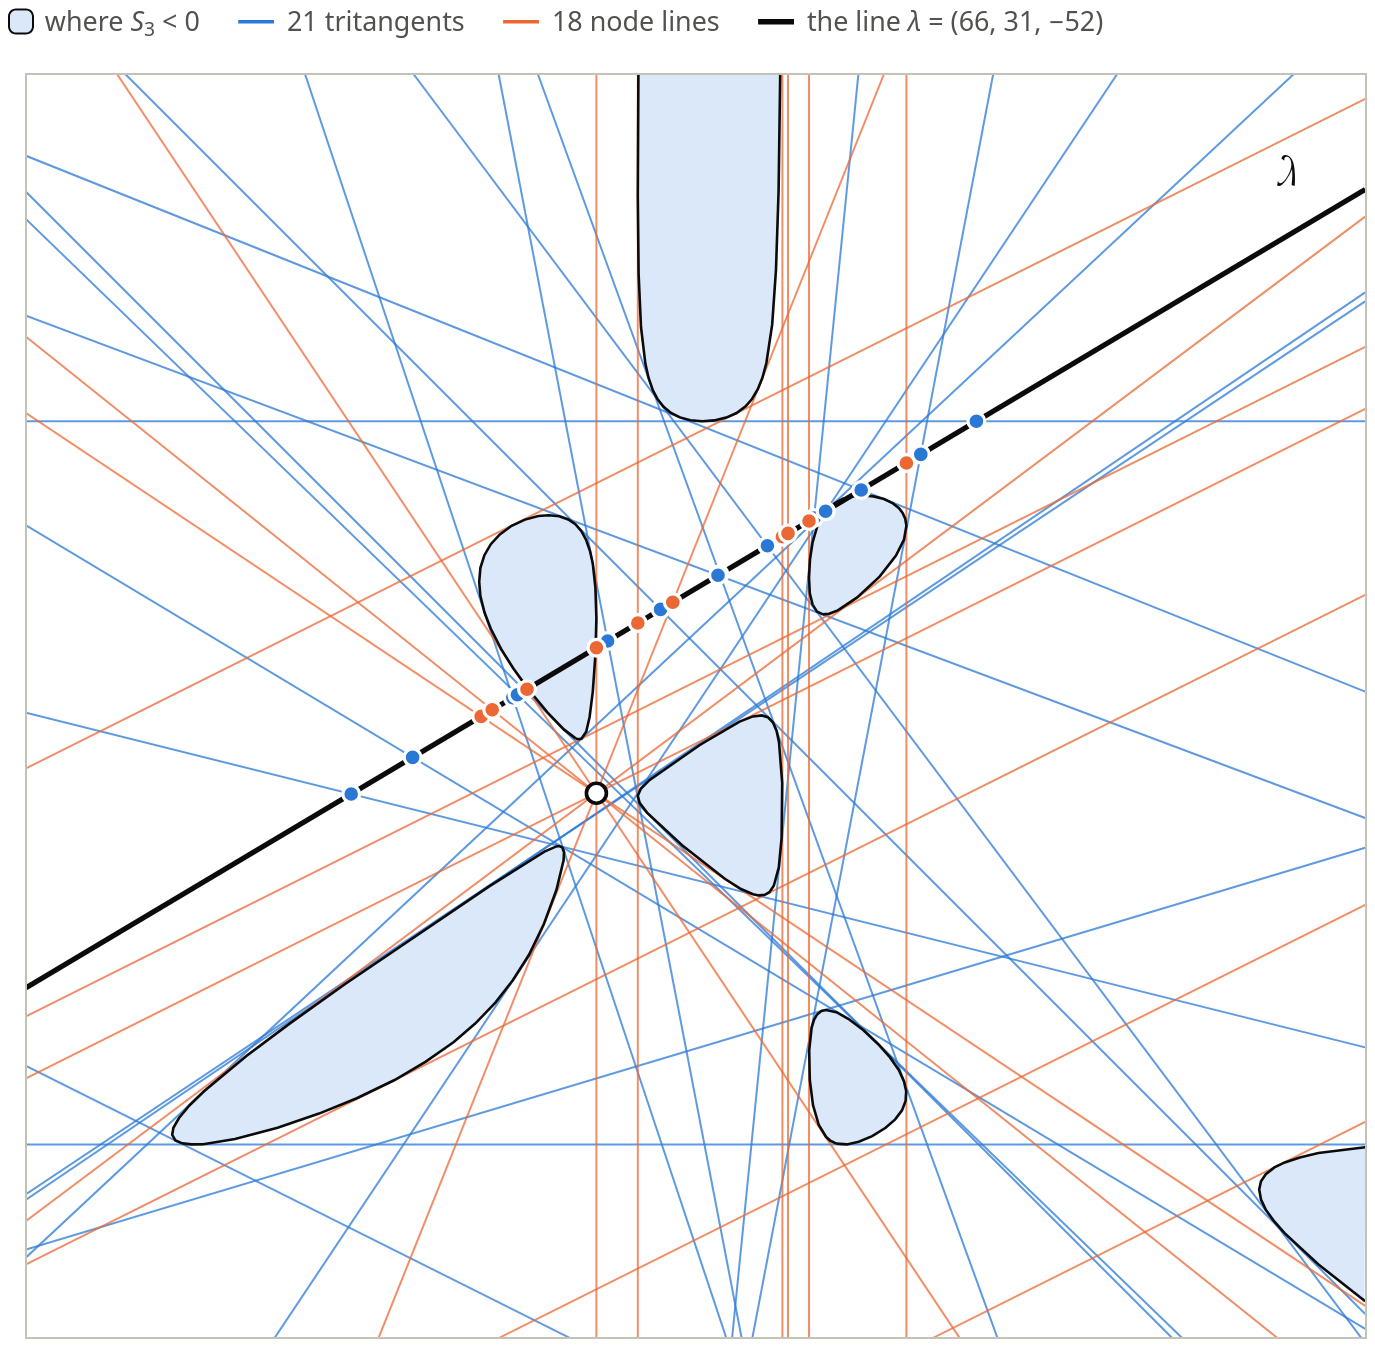
\includegraphics[width=0.78\linewidth]{figs/model.png}
\caption{The model that carries $C_{738}$, in the chart $z_0=1$ (its equation is in Section~\ref{sec:models}).  The outlined curve is the branch sextic; the surface has real points only over the unshaded region.  One of the three nodes is marked by an open circle; the other two are at infinity, where the vertical lines meet and where the parallel lines of slope $1/2$ meet.  The thin lines are the $21$ tritangents (blue) and $18$ node lines (orange).  The thick line is $\lambda=(66,31,-52)$; each dot where it crosses a thin line is a pair of rational points of $C_{738}$.}
\label{fig:model}
\end{figure}

For this to produce records the surface must have very many rational curves of low degree, all defined over $\Q$.  Elkies'
choice~\cite{ElkiesClay} is the surface $\X=\X_{163}$ of the next section, for which he wrote down a sextic with one node,
$43$ rational tritangents and $9$ rational node lines, hence $104$ forced points, and $1240$ rational
conics on which the sextic is a square.  Stoll~\cite{StollAvg} searched all lines of height at most $500$ on five such
sextics provided by Elkies, selecting lines by the size of $\prod_{p<200}\#C_\lambda(\F_p)/p$ before looking for points with
\texttt{ratpoints}~\cite{ratpoints}, and found $C_{642}$.

Two features of this strategy matter below.  First, nothing singles out one sextic: every degree-$2$ polarization of
$\X$ gives a different two-parameter family of genus $2$ curves on the same surface, and a genus $2$ curve
$C\subset\X$ is a line section of exactly one model, the one given by its own class.  Second, the forced points are only
the start.  $C_{642}$ lies on a model with $106$ forced points (see Table~\ref{tab:strata}) and has $642$ points;
$C_{738}$ lies on one with only $78$.

\section{The surface and its degree-2 polarizations}\label{sec:surface}

$\X_{163}$ is the K3 surface over $\Q$ of Picard number $20$ whose N\'eron--Severi lattice has discriminant $-163$,
\[
\NS(\X)\;\cong\;U\oplus E_8(-1)^2\oplus\begin{pmatrix}-2&-1\\-1&-82\end{pmatrix},\qquad
T_\X\cong\begin{pmatrix}2&1\\1&82\end{pmatrix},
\]
with every divisor class defined over $\Q$~\cite{ElkiesClay}.  It has complex multiplication by the maximal order of
$\Q(\sqrt{-163})$, and its point counts are governed by the weight-$3$ newform of level $163$ with that CM:
$\#\X(\F_p)=p^2+20p+1+a_p$.  We use this identity as a check on every model we construct.

The surface has an equation that needs no table of coefficients.  It is the surface that Shioda and Inose~\cite{ShiodaInose}
attach to $E\times E$, for $E$ the elliptic curve with complex multiplication by the maximal order of $\Q(\sqrt{-163})$, whose
$j$-invariant is $-640320^3$.  With $a=53360=640320/12$, Inose's elliptic fibration~\cite{Inose,ShiodaSandwich} of that surface is
\[
y^2 = x^3-3a^2x-\Bigl(t+\frac1t+2a^3+2\Bigr),
\]
with fibres of type $\mathrm{II}^*$ at $t=0$ and $t=\infty$; Elkies~\cite{ElkiesSI} gives this equation together with a
generator of its Mordell--Weil group, a section of height $163/2$.  The sextic of Elkies from which our computation starts
(Section~\ref{sec:models}) is a model of this surface over $\Q$, by a birational map that is explicit in both directions.  On
Elkies' sextic the zero section of the fibration is the exceptional curve of the node, each of the two fibres of type
$\mathrm{II}^*$ consists of lifts of eight of the lines on which the sextic is a square and of one conic, and the other fibres are
curves of degree $32$.  The map is given by forms of degree $32$ and $24$, its inverse by forms of degree $34$; both are in the repository~\cite{Repo} (directory \texttt{inose/}), with scripts that prove
that they are mutually inverse.

\subsection*{Models as lattice classes}
A degree-$2$ polarization is a nef class $D\in\NS(\X)$ with $D^2=2$ and no class $E$ with $E^2=0$, $E\cdot D=1$
(the condition for $|D|$ to have no base points~\cite{SaintDonat}).
Everything about the corresponding double plane that concerns us can be read off the negative definite lattice
$L=D^\perp$ of rank $19$ and determinant $326$:
\begin{itemize}\itemsep 1pt
\item the roots of $L$ (vectors of norm $-2$) are, up to sign, the effective combinations of contracted curves of
self-intersection $-2$, and the contracted curves themselves are the simple roots; so the root system of $L$ is the
ADE type of the singularities of the branch sextic;
\item the roots $E$ of $\NS(\X)$ with $E\cdot D=1$ are the components of the pullbacks of tritangents and node lines, possibly with contracted curves added.  They
correspond to the vectors of norm $-5/2$ in the nontrivial coset of $L$ in the projection of $\NS(\X)$ to $L\otimes\Q$;
counting them modulo the roots of $L$ gives the number of forced points;
\item the classes with $E^2=-2$, $E\cdot D=2$ that are irreducible (those that meet every curve of the first two kinds
non-negatively) are the lifts of the conics on which the sextic is a square, together with the pullbacks of any lines through two
nodes that are not node lines; and so on.
\end{itemize}
Because the discriminant group of $\NS(\X)$ is cyclic of odd prime order, two polarizations give isomorphic double planes if
and only if they lie in the same orbit of $O(\NS(\X))$.  The orbits of \emph{all} classes $D$ with $D^2=2$ correspond
bijectively to the isometry classes in the genus of $\langle 2\rangle\oplus E_8^2\oplus T_\X$ (as positive definite lattices),
by $D\mapsto D^\perp(-1)$ (this is Nikulin's theory of primitive embeddings and discriminant forms~\cite{Nikulin}), but not all of
them are polarizations.  A class $E$ with $E^2=0$, $E\cdot D=1$ exists exactly when
$D^\perp$ splits off a root, $D^\perp=\langle r\rangle\oplus M$ with $r^2=-2$: then $E=(D+r)/2$, and conversely $r=2E-D$.
These excluded classes correspond bijectively to the genus of $E_8^2\oplus T_\X$, which contains $M(-1)$; they are the elliptic
fibrations of $\X$ with a section, and the lattice $\langle 2\rangle\oplus E_8^2\oplus T_\X$ itself is one of them.  The mass of the
first genus is about $16{,}417.77$ and that of the second about $2.22$.  The root $r$ is unique up to sign, so
$\langle r\rangle\oplus M$ has twice as many automorphisms as $M$, and the polarizations carry mass
$16{,}417.77-2.22/2\approx 16{,}416.66$.  Every lattice has the automorphism $-1$, so there are more than $32{,}800$ models, and in
fact far more, because most of the mass sits on classes with large root systems and large automorphism groups.  A complete
enumeration is out of reach.

\subsection*{The census}
We sampled the genus with seven independent random walks along Kneser $3$-neighbours~\cite{Voight}, $9.9\times10^6$ steps
in all.  In the stationary distribution of such a walk a class has weight proportional to $1/|\mathrm{Aut}(L)|$, so a class with
$|\mathrm{Aut}(L)|=a$ is expected $606/a$ times, and the classes with few roots, which are the ones with small automorphism groups,
are found many times over.  A random walk cannot prove that a list is complete.  If the visits to a class were independent draws,
the class would be missed with probability about $e^{-606/a}$.  Successive steps of a walk are not independent, so this is a
heuristic and not a bound, but the visit counts behave much as it predicts: the $1141$ three-node classes whose automorphism group
was computed and has the generic order $16$ were visited $37.6$ times on average, where $37.9$ are expected, with variance $42.5$
(for independent draws the variance would equal the mean), and of the $193$ classes with one or two nodes, $185$ were found by each
of the seven walks separately and the other eight by six of them.  Table~\ref{tab:strata} summarizes the classes with at most three
contracted curves.  Every class in it was visited at least $4$ times, and every three-node class at least $10$ times.  On this
heuristic the classes at risk are those with many automorphisms: the estimated chance of missing a class is about $10^{-4}$ for
$a=64$, one in a hundred for $a=128$ and one in ten for $a=256$.  On this evidence the table should be complete for classes with small
automorphism groups, and it may lack classes with large ones.  We have not proved that it is complete, and nothing below depends
on it.  For every class it meets, the census records the
number of classes $E$ with $E^2=0$, $E\cdot D=1$; it is zero for all $53{,}361$ classes recorded, so every class counted in
the table is a polarization.

\begin{table}[h]
\centering\small
\begin{tabular}{llrcl}
\toprule
singularities of $B$ & roots & classes & forced points & remarks\\
\midrule
none & $\emptyset$ & $0$ & & no smooth sextic model seems to exist\\
one node & $A_1$ & $7$ & $104$--$108$ & Elkies' model ($104$); $C_{642}$ (on one with $106$)\\
two nodes & $A_1^2$ & $186$ & $86$--$96$ & \\
one cusp & $A_2$ & $8$ & $88$--$92$ & \\
three nodes & $A_1^3$ & $2192$ & $72$--$86$ & $C_{738}$ and $C_{654}$\\
node and cusp & $A_1+A_2$ & $550$ & $72$--$82$ & \\
\bottomrule
\end{tabular}
\caption{Degree-$2$ polarizations of $\X_{163}$ with at most three contracted curves, from the random-walk census.
Deeper strata are much larger (more than $13{,}000$ classes with four nodes were recorded) and have fewer forced points.}
\label{tab:strata}
\end{table}

The seven one-node models have $(\text{tritangents},\text{node lines})=(46,8)$ once, $(45,8)$ three times, $(44,9)$ twice, and
$(43,9)$ once; the last is Elkies' published sextic, and $C_{642}$ is a line section of one of the $(45,8)$ models.
Degtyarev~\cite{Degtyarev} has classified the smooth models of the K3 surfaces of Picard number $20$ and small discriminant;
his result for double planes stops at discriminant $116$, so it does not decide whether $\X_{163}$ has a smooth sextic model, but
for this same surface he finds more than three thousand configurations of lines on smooth quartic models.  The abundance of models
is not special to double planes.

The number of forced points falls as the root system grows.  The search of this note uses the models of the rows with one, two
and three nodes: all seven with one node, all $186$ with two, and $2188$ of the $2192$ with three.  The model of $C_{738}$ is an
unremarkable member of the three-node stratum, with $78$ forced points ($21$ tritangents and $18$ node lines), in the middle of
the range.

\section{The models}\label{sec:models}

The census gives lattices, not equations, and to search a model we need its sextic.  We obtain the sextics from a single one,
Elkies' sextic, by moving the polarization.  The computation finds the classes it constructs by itself; it does not use the
census.

\subsection*{The conic-pair construction}
Start from Elkies' model $w^2=S_E$,
\begin{align*}
S_E={}&3686400x_0^6+(-8697600x_1^2+2193664x_1x_2+11520x_2^2)x_0^4\\
&+(5130225x_1^4-1860100x_1^3x_2+138414x_1^2x_2^2-4180x_1x_2^3+9x_2^4)x_0^2\\
&-45144x_1^5x_2+19960x_1^4x_2^2-1672x_1^3x_2^3+40x_1^2x_2^4 ,
\end{align*}
which has its node at $(0:0:1)$.  We computed its rational conics on which $S_E$ is a square, with a rational
parametrization of each ($1241$ in our table).  A conic $q=0$ has two lifts to $\X$: if $S_E$ restricted to the conic is
$g^2$ and $G$ is a cubic form restricting to $g$, they are $\Gamma=\{q=0,\ w=G\}$ and $\Gamma'=\{q=0,\ w=-G\}$, both smooth
rational curves with self-intersection $-2$ and $\Gamma\cdot D_E=2$.

Two conics $q_1,q_2$ meet in four points of the plane, and at each of them the chosen lifts either agree ($G_1=G_2$) or
differ by sign.  If they agree at exactly three, then $\Gamma_1\cdot\Gamma_2=3$ and
\[
D'=\Gamma_1+\Gamma_2,\qquad D'^2=-2-2+2\cdot 3=2,\qquad D'\cdot\Gamma_i=1,
\]
is a new polarization of degree $2$.  It is nef because it is a sum of two irreducible curves each meeting it positively.
In the new double plane the two conics become the two lifts of a single tritangent line.

The sections of $\mathcal O(D')$ are the functions
\[
\frac{P+Q\,w}{q_1q_2},\qquad P \text{ a quartic form},\ Q \text{ a linear form},
\]
whose numerator vanishes on the other lifts $\Gamma_1'$ and $\Gamma_2'$, that is, $P\equiv QG_i \pmod{q_i}$ for $i=1,2$.
These are $9+9$ linear conditions on $15+3$ unknowns, of rank $15$, and the solution space has dimension $3=h^0(D')$.  A basis
$z_0,z_1,z_2$ gives the new map to $\PP^2$.  To find the new branch sextic we use that the Jacobian determinant of
$(z_1/z_0,z_2/z_0)$ with respect to affine coordinates $(x_1,x_2)$ of the old plane vanishes along the new ramification curve.
Multiplied by $w$ it changes sign under the new covering involution, and multiplied also by $z_0^3$ it becomes a form of the
right weight in the $z_i$:
\[
T \;=\; z_0^3\,w\,\det\frac{\partial(z_1/z_0,\,z_2/z_0)}{\partial(x_1,x_2)}
\;=\; w\,\det\begin{pmatrix} z_0&z_1&z_2\\ \partial_1z_0&\partial_1z_1&\partial_1z_2\\ \partial_2z_0&\partial_2z_1&\partial_2z_2\end{pmatrix},
\]
where $\partial_j=\partial/\partial x_j$ is taken on the surface, so that $\partial_jw=\partial_jS/(2w)$.  Then
$T^2=c\,S'(z_0,z_1,z_2)$ for a sextic form $S'$ and a nonzero constant $c$, and $w'=T/\sqrt c$ after scaling.
We determine the $28$ coefficients of $S'$ by exact linear algebra from a few hundred rational points of
$\X$ (points on other conics), and confirm the identity on fresh points.  For the model of $C_{738}$ we also verify it as an
identity of polynomials (see the worked example).

\subsection*{From Elkies' sextic to $2381$ models}
The construction is applied to every pair of conics that gives a model with at most three nodes.  The pairs are found, and
sorted into models, in the N\'eron--Severi lattice, which is computed from the sextic.
\begin{enumerate}\itemsep 1pt
\item \emph{Lines.}  An exhaustive search finds the lines of height at most $150$ on which $S_E$ is a square: $43$ tritangents
and $9$ node lines.  The $104$ components of their pullbacks and the exceptional curve of the node span a lattice of rank $20$
and discriminant $-163$, hence all of $\NS(\X)$, and from here on curves are handled through their classes.
\item \emph{Conics.}  The conics on which $S_E$ is a square are found modulo $41$, lifted to characteristic $0$ and verified
exactly.  The class of a lift of a conic is determined by its intersection numbers with the lifts of the lines.  An enumeration of
all classes $E$ with $E^2=-2$ and $0\le E\cdot D_E\le 2$ then shows that both tables are complete: the irreducible classes of degree
$1$ are the lifts of the $52$ lines, and those of degree $2$ are the lifts of the $1241$ conics.
\item \emph{Pairs.}  For each pair of lifts with $\Gamma_a\cdot\Gamma_b=3$ the roots of $D'^\perp$, where $D'=\Gamma_a+\Gamma_b$, are
counted.  They are among the classes just enumerated: a root $v$ of $D'^\perp$ has $|v\cdot D_E|\le 3$ by the Hodge index theorem
(because $D'\cdot D_E=4$), and $v\cdot D_E=3$ would make $D_E-D'+v$ a class of square $0$ and degree $1$, which a model does not
have.  The classes $D'$ with one, two or three roots, pairwise orthogonal, are kept: $380$, $3378$ and $13\,966$ classes on Elkies'
model.
\item \emph{Classes.}  For each $D'$ kept, the contracted curves and the components of the pullbacks of the tritangents and node
lines of the new model are found by a second enumeration, and the matrix of their intersection numbers is brought to a canonical
form under simultaneous permutations of its rows and columns.  In every case these classes generate $\NS(\X)$.  So two of the
classes $D'$ have the same canonical form if and only if an isometry of $\NS(\X)$ takes one to the other, that is, if and only if
they give isomorphic models (Section~\ref{sec:surface}).
\item \emph{The other one-node models.}  On Elkies' model the pairs give seven classes with one node, $180$ with two and $1531$
with three.  One of the seven is Elkies' model itself.  For each of the other six a sextic is constructed and the node is moved to
$(0:0:1)$; then steps 2 to 4 are repeated on it.  (Its lines are images of lines and conics of Elkies' model, and the enumeration of
step 2 confirms that none is missing.)  No further class with one node appears:
the seven one-node models are closed under the construction.  Together they give $186$ classes with two nodes and $2188$ with
three.
\item \emph{Sextics.}  For each class one pair of conics is chosen, on Elkies' model whenever the class occurs there, and the
sextic is constructed.  Several things are checked.  The lines and conics of the old model whose classes have degree $1$ or $0$
for $D'$ must be mapped to lines on which the new sextic is a square and to singular points of it; the new sextic must have the number
of nodes and of lines that the lattice gives; and its point counts modulo the primes between $47$ and $100$ must agree with the CM form.
\end{enumerate}
The models constructed are therefore the seven models with one node that are reached from Elkies' model by conic pairs, and all the
models with two or three nodes that are sums of two conics on one of these seven: $7+186+2188=2381$ models.  The census of
Section~\ref{sec:surface} has the same seven classes with one node and the same $186$ with two, and it has $2192$ with three: the
$2188$ constructed here and four more (the script \texttt{census.m} compares the lattices).  These four are not sums of two conics on a one-node model.  (A sum of two conics on a
one-node model $D_0$ always has $D'\cdot D_0=4$, and for each of the four the lattice shows that no one-node class of the census
has $D'\cdot D_0\le 4$.)  There is no deeper obstruction.  They can be written down by another route, for instance starting from a
model with two or three nodes, or as a sum of three curves; we have not done that, so these four are the only three-node classes
of the census that are not searched.  The whole construction takes $7$ minutes.

\subsection*{Minimal coordinates}
The height of a line depends on the coordinates, so the sextic that comes out of the construction is replaced by a minimal and
reduced one, computed with Magma's \texttt{MinRedTernaryForm}~\cite{ElsenhansStoll}: a form $S(Mz)/c$, with $M$ an invertible
rational matrix, that is minimal at every prime and whose coefficients are then made small by a unimodular change of variables.
The effect on a search by height can be large.  Elkies' sextic $S_E$ is itself not minimal at the prime $2$: its minimal form has
largest coefficient $35\,356$ where $S_E$ has $8\,697\,600$, and the $52$ lines on which it is a square have height at most $37$
there, against $148$.  Of the $2380$ sextics that the construction produces, $397$ are not minimal as they come out.
A minimal sextic is not unique, however, and \texttt{MinRedTernaryForm} returns one that depends on the coordinates it is given.
For example, the sextic $S$ of the one-node model \texttt{b5} of our list has largest coefficient $6984$, and
$S(z_0-z_2,\,z_0+z_2,\,z_1-z_2)/4$ is another integral sextic for the same model, with largest coefficient $5134$.  The
change of coordinates has determinant $2$, which the division by $4$ compensates exactly ($2^6=4^3$), so the second sextic is
minimal as well.  A line has different heights on the two, so the set of lines of height at most $400$
depends on which minimal sextic is used (Section~\ref{sec:results}).  The constant $c$ matters: multiplying $S$ by a
number that is not a square replaces the double plane $w^2=S$ by a quadratic twist, a different surface over $\Q$.  We divide
only by squares, and the certificate below would detect a twist, because on a twist the sextic is no longer the square of a
polynomial with rational coefficients on the lines listed.

\subsection*{The list of models, and a certificate for it}
The search uses the $2381$ sextics: $7$ with one node, $186$ with two and $2188$ with three.  They are in the file
\texttt{data/models.txt}, each with its singular points and the lines on which it is a square.  The script \texttt{models.m}
verifies every one of them from that file alone, independently of the construction, by the argument given below for the model of
$C_{738}$.  The singular points of the sextic are the nodes listed and no others.  The sextic is the square of a polynomial with
rational coefficients on each line listed.  The lifts of these lines and the contracted curves span a lattice of rank $20$ and
discriminant $-163$, which is therefore the whole N\'eron--Severi lattice, so the surface is $\X_{163}$ and every class is defined
over $\Q$.  And the irreducible classes $E$ with $E^2=-2$, $E\cdot D=1$ are exactly the lifts, so the list of lines is complete.
The script then computes the lattice $D^\perp$ of each sextic and shows that no two of them are isometric: the $2381$ sextics are
$2381$ different models.  This confirms, by another method, the classification by canonical forms used in the construction.

\subsection*{Worked example: the model of $C_{738}$}
Take the conics
\begin{align*}
q_1&=3400x_0^2-3150x_0x_1+54x_0x_2-5400x_1^2+551x_1x_2-9x_2^2,\\
q_2&=5760x_0^2-5896x_0x_1-936x_0x_2-209x_1^2-458x_1x_2-9x_2^2
\end{align*}
of Elkies' model, the pair that the construction chooses for this class; the cubic forms $G_1,G_2$ that define their lifts are
in Appendix~\ref{app:map}.
The conics meet in one rational point and three points conjugate over a cubic field; the lifts agree at the three conjugate
points and differ at the rational one, so $\Gamma_1\cdot\Gamma_2=3$.  The lattice class of $D'=\Gamma_1+\Gamma_2$ has
root system $A_1^3$, with $21$ tritangents and $18$ node lines.  Solving the linear conditions and reducing gives three
sections $z_i=A_i+B_iw$ (the common denominator $q_1q_2$ is dropped), with linear forms $B_i$ and quartic forms $A_i$
that are also listed in Appendix~\ref{app:map}.
\begin{figure}[ht]
\centering
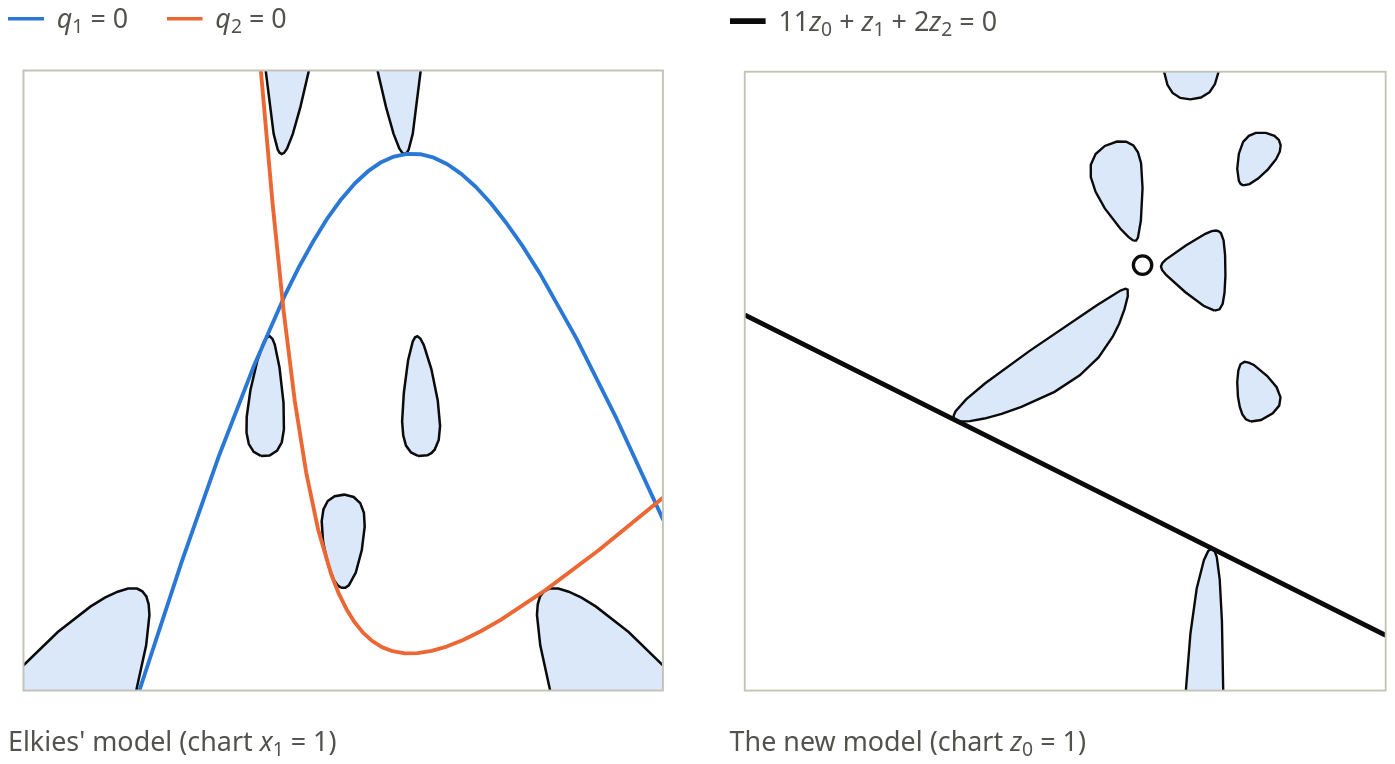
\includegraphics[width=0.92\linewidth]{figs/pair.png}
\caption{Two conics become one line.  Left: Elkies' sextic with the conics $q_1=0$ and $q_2=0$; each touches the sextic wherever it meets it.  Right: the three-node model built from them.  The chosen lifts $\Gamma_1$, $\Gamma_2$ of the two conics to the surface are mapped onto the two halves of the tritangent $11z_0+z_1+2z_2=0$.  The map involves $w$: it is a map of the surface, not of the plane.}
\label{fig:pair}
\end{figure}

In these coordinates the new model is $w'^2=S_{3}(z_0,z_1,z_2)$ with
\begin{align*}
S_{3}={}&25z_0^6+(-1930z_1+3240z_2)z_0^5+(969z_1^2-1734z_1z_2+1996z_2^2)z_0^4\\
&+(5752z_1^3-6326z_1^2z_2-996z_1z_2^2-864z_2^3)z_0^3\\
&+(2748z_1^4-1328z_1^3z_2-3588z_1^2z_2^2+960z_1z_2^3-176z_2^4)z_0^2\\
&+(-144z_1^5+216z_1^4z_2-548z_1^3z_2^2+1376z_1^2z_2^3+16z_1z_2^4)z_0\\
&+36z_1^6+12z_1^5z_2-311z_1^4z_2^2-52z_1^3z_2^3+676z_1^2z_2^4 .
\end{align*}
The statement is exact.  In the chart $x_0=1$, with $T$ the determinant displayed above,
\[
S_3(z_0,z_1,z_2)\;=\;\tfrac1{16}\,T^2\qquad\text{in }\ \Q(x_1,x_2)[w]/(w^2-S_E),
\]
an identity of polynomials; the script \texttt{verify.py} of the repository~\cite{Repo} checks it, together with the congruences
$S_E\equiv G_i^2$ and $A_j\equiv B_jG_i$ modulo $q_i$ that express the vanishing conditions.  In particular, for every rational
point $(x_0:x_1:x_2;w)$ of Elkies' model, $S_3(A_0+B_0w,\,A_1+B_1w,\,A_2+B_2w)$ is a rational square.  For instance, the line $x_2=0$ is a tritangent of Elkies' sextic, $S_E(x_0,x_1,0)=x_0^2(1920x_0^2-2265x_1^2)^2$.
Its lift $w=x_0(1920x_0^2-2265x_1^2)$ is mapped to the single point $(0:2:1)$: it is one of the three contracted curves.
On the other lift, the point $(1:1:0)$ with $w=345$ maps to $z=(118:-118:-75)$, where $S_3=7570880^2$.  The sextic $S_3$ is irreducible with exactly three singular points, the nodes
\[
(0:0:1),\qquad (0:2:1),\qquad (2:-2:-1),
\]
it is a square on exactly $21+18$ lines, as the lattice predicts ($15$ of the node lines pass through one node, and the other
three are the sides of the triangle of nodes), and its point counts match the CM form.  It is already minimal and reduced.  Its largest coefficient is $6326$, close to the median of the largest coefficient
over the $2381$ sextics, which is $6073$.

\emph{A certificate for the model.}  These statements, and the identification of the surface, can be checked without the
construction.  Appendix~\ref{app:magma} is a short Magma script that proves them from $S_3$ and the list of the $39$ lines alone.
The three nodes are the only singular points.  The $78$ components of the pullbacks of the lines and the three contracted curves
have an intersection matrix of rank $20$ and discriminant $-163$; so they generate the N\'eron--Severi lattice, the Picard number
is $20$, and every class is defined over $\Q$.  Over $\overline\Q$ the surface is therefore $\X_{163}$: a complex K3 surface of
Picard number $20$ is determined up to isomorphism by its oriented transcendental lattice~\cite{ShiodaInose}, and there is only one
positive definite even binary form of determinant $163$.  The lattice computation also identifies the surface over $\Q$, so it
confirms what the construction gives directly (an explicit map over $\Q$ from Elkies' model).  Let $\varphi$ be an isomorphism
over $\overline\Q$ between two such surfaces on both of which every divisor class is defined over $\Q$.  For $\sigma$ in the Galois
group, $\varphi^{-1}\circ\sigma(\varphi)$ is an automorphism that acts trivially on the N\'eron--Severi lattice.  On the
transcendental lattice it acts by a Hodge isometry, which here can only be $\pm1$ (the lattice is an ideal of $\Q(\sqrt{-163})$, whose
only units are $\pm1$), and it must act trivially on the discriminant group $\Z/163$, as it does on that of the N\'eron--Severi
lattice; so it acts trivially on all of $H^2$ and is the identity.  Hence $\sigma(\varphi)=\varphi$ for all $\sigma$, and
$\varphi$ is defined over $\Q$.
Enumeration in that lattice shows that $S_3$ is a square on exactly $39$ lines and on exactly $810$ conics.  And $\#\X(\F_p)$
agrees with the CM newform at the $32$ primes $41\le p<200$ of good reduction for the model.

Finally, the line $\lambda=(66,31,-52)$, that is $66z_0+31z_1-52z_2=0$, is parametrized by
$(z_0:z_1:z_2)=(6x-2:4x+16:10x+7)$, and
\begin{align*}
S_3(6x-2,\,4x+16,\,10x+7)=64\,\bigl(&743425x^6-16144220x^5+60026500x^4\\
&+172162750x^3+40133975x^2-46160230x+6838225\bigr).
\end{align*}
So $C_{738}=C_\lambda$.  In Elkies' plane the image of the same curve has degree $D'\cdot D_E=4$; it is not a line there.  A curve
isomorphic to it could still be a line section of another model, so we checked that directly.  On none of the other $2380$ sextics
of the list is $C_{738}$ isomorphic, even over $\overline\Q$, to the section by any line, rational or not, and on $S_3$ the line
$\lambda$ is the only one.  The proof is a computation.  Two binary sextics with nonzero discriminant define isomorphic curves over
$\overline\Q$ exactly when their Igusa--Clebsch invariants agree as points of the weighted projective space $\PP(2,4,6,10)$, so the
lines in question are the solutions of three polynomial equations in the coefficients of the line, together with the condition
that the discriminant of the section is not zero.  The script \texttt{linesection.m} treats all lines, in three charts, and shows
for each of the other sextics that the system has no solution over $\overline\Q$ (by a Gr\"obner basis, and a second time by
resultants); on $S_3$ it has exactly one solution.

\section{Searching a model}\label{sec:search}

A model has $2.1\times10^8$ lines of height at most $400$, and the $2381$ sextics together have $5.1\times10^{11}$.  Reducing the
sextic of a line and counting its rational points, even to a small height bound, costs a millisecond or two, which is far too much
to do for every line.  The lines are therefore ranked first, by a count that costs about a tenth of a microsecond per line.

\subsection*{The score of a line}
By a \emph{surface point of height at most $H$} we mean a point $(z_0:z_1:z_2)$ of the plane with coprime integer coordinates
of absolute value at most $H$ at which $S$ is the square of a rational number, zero included.  It is counted once, although two
points of the surface lie over it when $S\ne0$.  A surface point on a line $\lambda$ is a rational $x$-value of the curve
$C_\lambda$, so a line with many surface points of small height is a line whose curve has many points of small height.  The
\emph{score} of $\lambda$ is the number of surface points of height at most $4000$ on $\lambda$, not counting those on the lines
on which $S$ is a square: every line meets each of those lines, so they add the same forced points to every score.

The score of every line of height at most $400$ is computed in two steps, without looking at any line by itself.  First the surface
points are listed.  For each pair $(z_1,z_2)$ the values $S(z_0,z_1,z_2)$ with $|z_0|\le 4000$ are sieved for squares modulo
composite moduli built from small prime powers, $512$ values of $z_0$ at a time, and the survivors are tested exactly.  A model
has between half a million and a little over two million such points (on average $1.8$, $1.5$ and $1.3$ million for one, two and three
nodes).  Then, for each point $p$, the lines of height at most $400$ through $p$ are enumerated (they are the vectors of small
sup-norm in a lattice of rank $2$, the integer vectors orthogonal to $p$), and a counter for each of these lines is incremented in
a table with one entry for every line of height at most $400$.  The two steps together take $0.11$ microseconds of processor
time per line.

\subsection*{The stages}
The settings are the same for every model.
\begin{enumerate}\itemsep 1pt
\item Lines through a singular point are discarded (their curves have genus at most $1$), and the lines with a score of at least
$40$ are kept: on average $7400$ lines on a model with one node, $4300$ with two nodes and $2600$ with three.
(Models with fewer nodes have more lines with many points; see Section~\ref{sec:results}.)
\item For each line kept, $S$ is restricted to the line and the sextic obtained is reduced, with \texttt{hyperellred} of
PARI/GP; then the rational points of height at most $2000$ are counted.  For the curves with at least $250$ of them the points of
height at most $10^4$ are counted, and for those with at least $330$ of these, the points of height at most $10^5$.
\item For each curve with at least $440$ points of height at most $10^5$, the set of these points is closed under the four-point
relation of Section~\ref{sec:closure}.  The number of points reported for a curve is the number after closure.
\end{enumerate}
The point counts use a sieve over the pairs $(a,c)$ with $x=a/c$: for composite moduli $M$ built from small primes, bit tables
record for which $(a,c)$ modulo $M$ the value $c^6f(a/c)$ is a square, $512$ numerators are processed at a time, and
survivors are tested exactly.  On two threads a three-node model takes about $20$ seconds, a two-node model about
$35$ and a one-node model about $120$ (medians).

\subsection*{What happens on the model of Section~\ref{sec:models}}
The sextic $S_3$ has $1\,328\,965$ surface points of height at most $4000$ off its $39$ special lines.  Of the lines of height
at most $400$ that pass through no node, $249\,542$ contain at least $15$ of them and $2460$ contain at least $40$; these are
the lines kept.  The line $(66,31,-52)$ has the highest score of all, $112$, and it is first at every later stage:
\begin{center}
\begin{tabular}{lrrrrr}
\toprule
 & score & \multicolumn{3}{c}{points of height at most} & after closure\\
 & & $2000$ & $10^4$ & $10^5$ & \\
\midrule
the line $(66,31,-52)$ & $112$ & $424$ & $536$ & $662$ & $738$\\
best other line of the model & $95$ & $310$ & $346$ & $376$ & \\
\bottomrule
\end{tabular}
\end{center}
(The counts refer to the reduced sextic used in the search, which differs from the equation of the abstract by
$x\mapsto -2x$; in the coordinates of the abstract the last two are $554$ and $666$.)  Of the $2460$ curves, $27$ have at
least $250$ points of height at most $2000$, four have at least $330$ of height at most $10^4$, and one has at least $400$ of height
at most $10^5$ (Figure~\ref{fig:funnel}).  So the model is ordinary, and $C_{738}$ is a single outlier that is unmistakable from the score on
(Figure~\ref{fig:score}).  The whole search of this model, closure included, takes $22$ seconds on two threads.

\begin{figure}[ht]
\centering
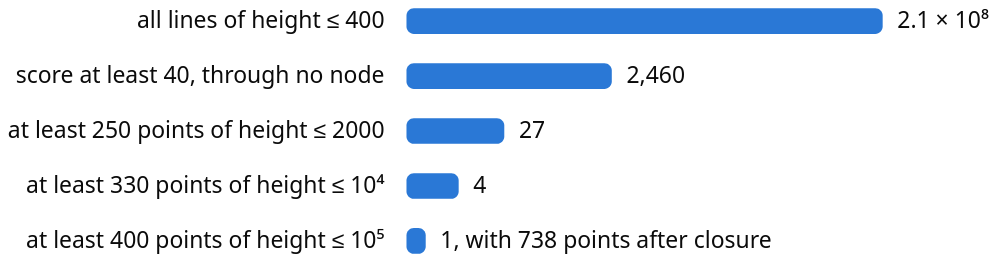
\includegraphics[width=0.9\linewidth]{figs/funnel.png}
\caption{The search on the model of $C_{738}$, stage by stage (bar lengths are logarithmic).}
\label{fig:funnel}
\end{figure}

\begin{figure}[ht]
\centering
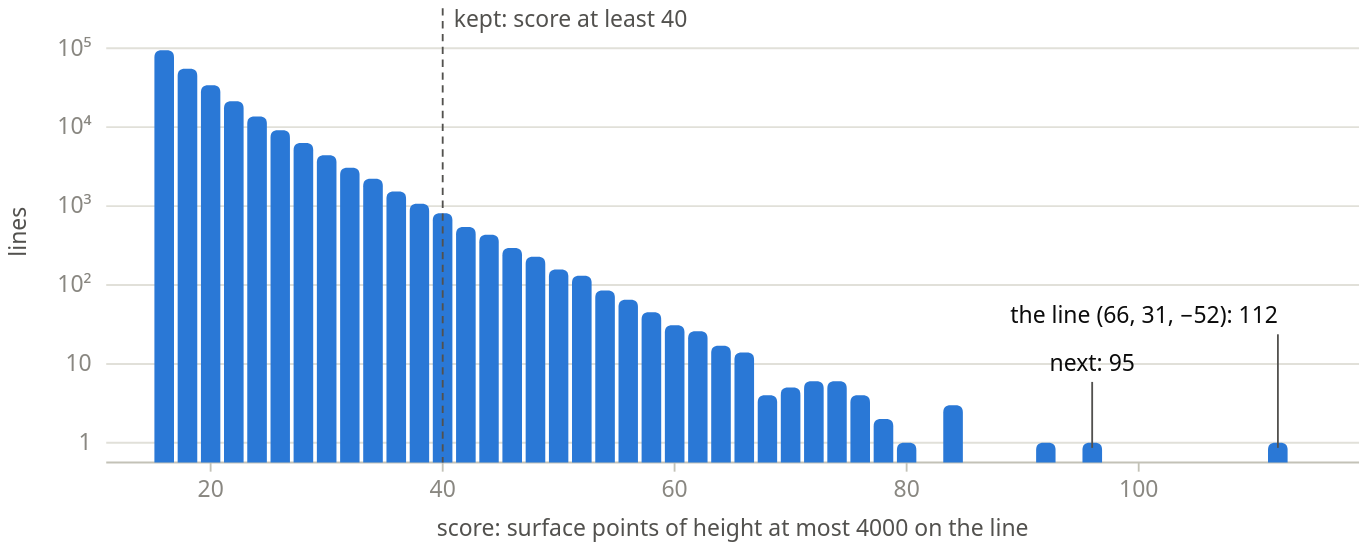
\includegraphics[width=0.9\linewidth]{figs/score.png}
\caption{The scores of the lines of height at most $400$ on the model of $C_{738}$: the number of lines, on a logarithmic scale, with a given number of surface points of height at most $4000$ (lines through a node and lines with fewer than $15$ points are not shown).  The $2460$ lines with a score of at least $40$ are kept.}
\label{fig:score}
\end{figure}

How far do lines, conics and cubics account for the points (Figure~\ref{fig:xvalues})?  The $39$ special lines give $39$ distinct forced
$x$-values.  The complete conic table of $S_3$ has $810$ conics, as the lattice predicts, and $62$ of them meet the line in rational
points, at $95$ distinct $x$-values because many of them share points on the line.  For the next layer we tabulated $21250$ cubics
on which $S_3$ is a square (those that pass through at most one of the three nodes).  A line meets a cubic in three points, and $360$ of these cubics cross $\lambda$ in a rational point, at
$137$ distinct $x$-values, of which $74$ are on no line or conic.  Lines, conics and cubics together account for $206$ of
the $369$ $x$-values; the other $163$ are not accounted for by the tabulated curves.  They may lie on curves of degree four and more or on cubics
missing from the table, or on no rational curve of low degree at all.  The search uses none of these tables: it counts points, whatever puts them there.

\begin{remark*}
The selection is a heuristic and loses curves: a line of height at most $400$ whose curve has many points is missed if its score
is below $40$, or if one of its counts falls below a threshold.  The record line is far from these limits.  The margin is
small for weaker curves, however.  On the model above, the four curves with at least $330$ points of height at most $10^4$ have
ranks $1$, $2$, $34$ and $2105$ by score among the $2460$ lines kept: the last has score $41$, just above the bound, and $262$
points of height at most $2000$, against a threshold of $250$.  Its curve has $372$ points of height at most $10^5$; lines of that
quality with a score of $39$ are not seen.  Section~\ref{sec:results} measures what is lost in the whole search.
\end{remark*}

\section{The cubic closure}\label{sec:closure}

The point counts of the search stop at height $10^5$, and going much further is expensive.  On curves of rank $20$ or so there is
a far cheaper way to find the larger points, because the large points are tied to the small ones by simple relations in the Jacobian.  The idea goes back to Stoll's search~\cite{StollAvg},
who tested whether five known points lie on a cubic.

Let $C\colon y^2=f(x)$ with $f$ of degree $6$ and leading coefficient $f_6$, and let $D_\infty$ be the divisor of the two
points at infinity.  Take four known points $P_i=(x_i,y_i)$ with distinct $x_i$ and let $p(x)$ be the cubic polynomial with
$p(x_i)=y_i$.  Let $p_3$ be the leading coefficient of $p$ and suppose $p_3^2\ne f_6$.  Then the function $y-p(x)$ has polar divisor
$3D_\infty$, so it has six zeros: the $P_i$ and two more points $P_5,P_6$, with
\[
P_5+P_6\;\sim\;3D_\infty-(P_1+P_2+P_3+P_4).
\]
Their $x$-coordinates are the roots of the quadratic $r$ in
\[
p(x)^2-f(x)=(p_3^2-f_6)\,(x-x_1)(x-x_2)(x-x_3)(x-x_4)\,r(x),
\]
\emph{If the discriminant of $r$ is a square, $P_5$ and $P_6$ are rational
points}, with $y=p(x)$.  (If $p_3^2=f_6$, which requires $f_6$ to be a square, then $y-p(x)$ has a pole of order less than $3$ at one of the two points
at infinity.  As a section of $\mathcal O(3D_\infty)$ it vanishes there once or twice, the remaining factor has degree one or zero
accordingly, and the relation between divisor classes is the same, with that point at infinity counted among the six zeros.)  Replacing some $P_i$ by their hyperelliptic conjugates changes the cubic, so each set of four
$x$-values gives eight tests.  The closure runs over all four-element subsets of the known points and all sign patterns,
adds the points found, and repeats until nothing new appears.  With $n$ known $x$-values this is $n^4/3$ tests, each of them
the question whether one rational number is a square.  Almost all of them are decided without computing that number.  Let $p$ be
a prime of good reduction at which $f$ has a root, and let $W$ be the Weierstrass point of the curve over $\F_p$ above that root.
The six points in which a cubic $y=p(x)$ meets the curve satisfy $\sum_i[P_i-W]=0$ in $J(\F_p)$.  So four points can have two
rational partners only if minus the sum of their four classes $[P_i-W]$ is a sum of two such classes.  The
classes of the known points are computed once for the primes $p\le 257$ of this kind, the test for a set of four is then a table
lookup for each prime, and the sets that pass for all of them (about one in five hundred on $C_{738}$) are tested exactly.  Two variants are
run as well: tangent relations, in which the cubic meets the curve twice at a known point, and, when $f_6$ is a square, relations
through the points at infinity.

\begin{figure}[ht]
\centering
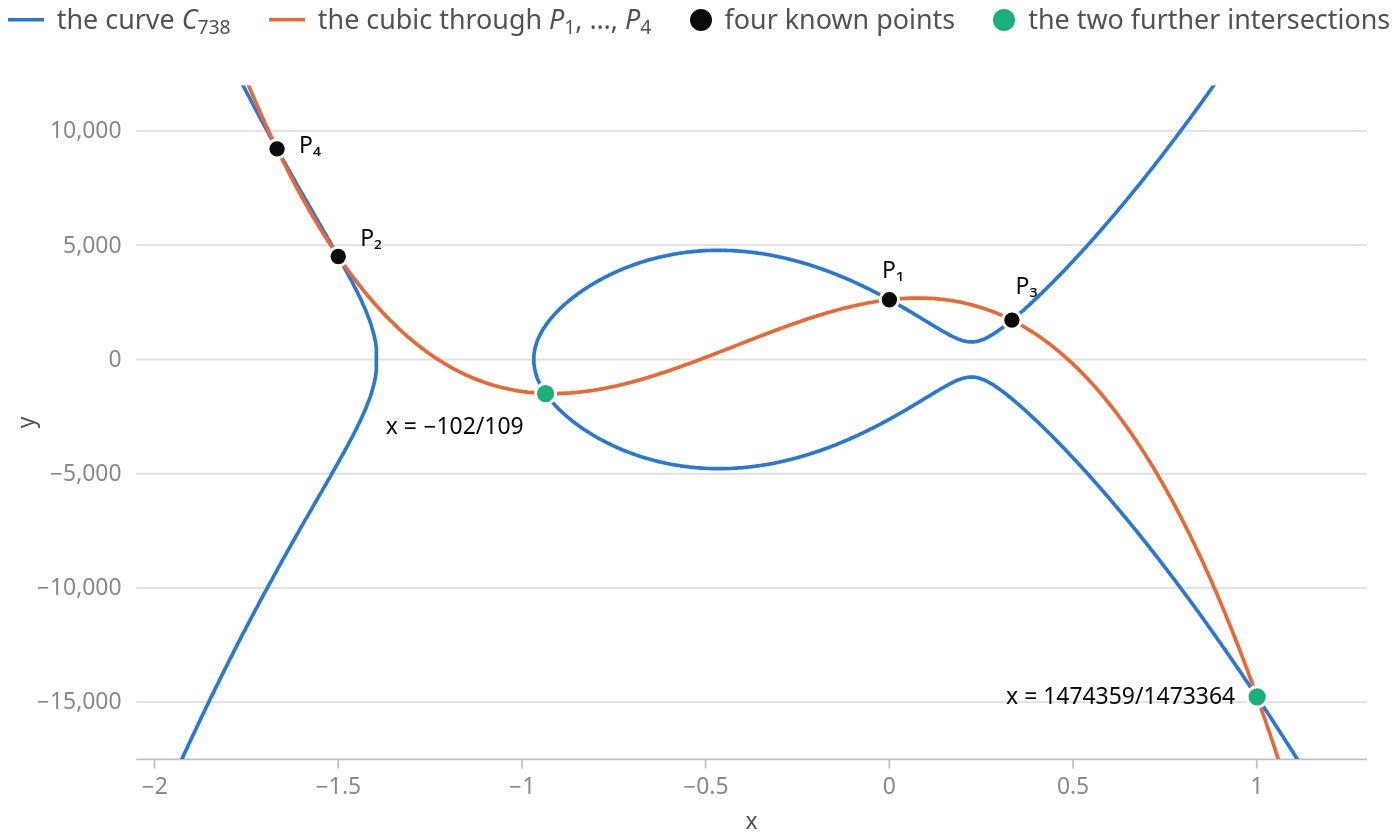
\includegraphics[width=0.9\linewidth]{figs/closure.png}
\caption{The curve $C_{738}$ (blue), the cubic through four known points $P_1,\dots,P_4$ of height at most $5$ (orange), and the two further intersection points (green): $x=-102/109$, which was known, and $x=1474359/1473364$, whose height is far beyond the point counts of the search.  The formulas are in the worked example below.}
\label{fig:closure}
\end{figure}

Unlike the five-point test, this finds two new points from four known ones and needs no fifth point on the cubic.  There is
a second difference.  Write $[P]$ for the class of $P-\iota P$ in $J(\Q)$, where $\iota$ is the hyperelliptic involution.  The
relation above gives
\[
[P_5]+[P_6]=-\bigl([P_1]+[P_2]+[P_3]+[P_4]\bigr),
\]
so the \emph{sum} of the two new classes lies in the subgroup generated by the classes of the known points, but $[P_5]$ and
$[P_6]$ separately need not.  (For five known points on a cubic the class of the sixth point is minus the sum of theirs, so that test
stays inside the subgroup.)  The closure can therefore enlarge the subgroup, and it does: the five $x$-values of the
certificate at the end of this section give classes generating a subgroup of rank at most $5$, and their closure is the whole
list, which generates rank $21$.

\subsection*{Worked example: the points of $C_{738}$}
The numbers of known points by height, on the equation of the abstract:
\begin{center}
\begin{tabular}{lrrrrrrrrr}
\toprule
height at most & $10$ & $10^2$ & $10^3$ & $10^4$ & $10^5$ & $10^6$ & $10^7$ & $10^8$ & $10^9$\\
\midrule
points & $36$ & $188$ & $390$ & $554$ & $666$ & $712$ & $732$ & $736$ & $738$\\
\bottomrule
\end{tabular}
\end{center}
The columns up to $10^7$ are sieve counts; the sieve to $10^7$ finds no point that the closure had not already found.
Starting from the $333$ $x$-values of height at most $10^5$, the first pass of the closure runs through the $5.0\times 10^8$
four-element subsets in a few seconds and finds the other $36$ $x$-values, of heights between $1.06\times10^5$ and $1.86\times10^8$;
the second pass finds nothing.  The same $369$ $x$-values are reached from the points of height at most $10^3$ or $10^4$ alone.
The largest point has
\[
x=\frac{185880347}{11934737}.
\]

Here is one relation explicitly.  The curve has the points
\[
P_1=(0,\,2615),\quad P_2=\Bigl(-\tfrac32,\ \tfrac{36025}{8}\Bigr),\quad P_3=\Bigl(\tfrac13,\ \tfrac{46475}{27}\Bigr),\quad
P_4=\Bigl(-\tfrac53,\ \tfrac{248815}{27}\Bigr),
\]
and the cubic through them is
\[
p(x)=-\tfrac{25477}{3}x^3-\tfrac{96152}{9}x^2+\tfrac{5471}{3}x+2615 .
\]
Then
\[
p(x)^2-f(x)=\tfrac{2}{81}\;x\,(2x+3)(3x-1)(3x+5)\,(109x+102)\,(1473364x-1474359),
\]
so the cubic meets the curve again at
\[
x=-\frac{102}{109}\qquad\text{and}\qquad x=\frac{1474359}{1473364},\quad y=-\frac{47232542363775629256305}{1473364^3}.
\]
The first of these has height $109$ and was known.  The second has height about $1.5\times10^6$ and lies far beyond the point
counts of the search.  Four points of height at most $5$ have produced it.

\subsection*{A certificate for the $738$ points}
No point count is needed to check the result.  The curve has the ten points
\[
(0,\pm 2615),\quad \Bigl(-\tfrac12,\ \pm\tfrac{38115}{8}\Bigr),\quad \Bigl(\tfrac12,\ \pm\tfrac{34475}{8}\Bigr),\quad
\Bigl(-\tfrac32,\ \pm\tfrac{36025}{8}\Bigr),\quad \Bigl(\tfrac13,\ \pm\tfrac{46475}{27}\Bigr),
\]
the points with $x$ of height at most $3$, and their four-point closure is the whole list of $369$ $x$-values.  So these five
$x$-values, together with the closure rule, are a certificate for the claim of $738$ points: anyone can regenerate every point from
them and check each one on the curve.  The HTML version of this note, at \url{https://math.mit.edu/~drew/g2ratpoints738.html}, contains a short program
(\texttt{closure.js}, exact integer arithmetic) that does this in a browser for any curve $y^2=f(x)$ with $f$ of degree $5$ or $6$
and any rational starting points; it verifies the starting points, runs the closure and checks every point it finds.  For each
point it records the four points and the cubic that first produced it, so every point can be traced back to the five starting
values.  Points with $y=0$ are used like the others, and
rational points at infinity, when the curve has them, are known from the start and the relations through them are found as well.  With the restriction that each relation uses two of the $16$ known points of smallest height it
tries $7.8\times10^6$ sets of four and returns the $369$ $x$-values in well under a minute.

\section{The curve}\label{sec:curve}

We collect what has been verified about $C_{738}$; write $f$ for its sextic and $J$ for its Jacobian.
\begin{itemize}\itemsep 2pt
\item \emph{Points.}  $369$ $x$-values, each checked exactly, none at infinity ($f_6=743425$ is not a square) and none with
$y=0$.
\item \emph{Arithmetic of $f$.}  $f$ is irreducible modulo $67$, and modulo $47$ and $59$ it has irreducible factors of degrees
$1,5$ and $1,2,3$.  So its Galois group is transitive and contains a $5$-cycle and a transposition (the cube of an element of cycle
type $1,2,3$), and is therefore $S_6$; in particular $J(\Q)[2]=0$.  The discriminant of $f$ is
$-2^9\,3^6\,5^{10}\,7^9\,11^8\,13^2\,29^2\,37^3\,61^2\,137^3$ times a $28$-digit prime.
\item \emph{Torsion and endomorphisms.}  $\#J(\F_{43})=3022=2\cdot 1511$ and $\#J(\F_{47})=3537=3^3\cdot 131$ are coprime, so
$J(\Q)$ is torsion-free.  Since the Galois group of $f$ is $S_6$, a theorem of Zarhin~\cite{Zarhin} gives
$\mathrm{End}(J_{\overline\Q})=\Z$.  Hence $J$ is absolutely simple, and the only automorphisms of the curve over $\overline\Q$ are
the identity and the hyperelliptic involution.  (A check that does not use Zarhin's theorem: the characteristic polynomial of
Frobenius at $43$ is $x^4+22x^3+204x^2+946x+1849$, and the characteristic polynomials of its powers up to the $92$nd are
irreducible.  A splitting of $J$ over an extension of $\F_{43}$ would make one of the first $30$ reducible, so the reduction of
$J$ modulo $43$ is absolutely simple.)
\item \emph{Rank.}  Put $P_0=(0,2615)$ and let $\Lambda\subset J(\Q)$ be the subgroup generated by the classes $[P-P_0]$ of the
known points $P$; it is also the subgroup generated by all differences of known points.  Its rank is exactly $21$.  The lower
bound is unconditional.  Take the $20$ points with
\[
x=-\tfrac12,\ \tfrac12,\ -\tfrac32,\ \tfrac13,\ \tfrac43,\ -\tfrac34,\ \tfrac14,\ \tfrac52,\ -\tfrac53,\ -\tfrac25,\ -\tfrac15,\ -6,\
-\tfrac73,\ -\tfrac75,\ \tfrac47,\ 8,\ \tfrac18,\ -\tfrac{11}6,\ \tfrac9{11},\ \tfrac{12}5
\]
and the point $\iota P_0$.  Their $21$ classes $[P-P_0]$ are independent, and they are in fact a basis of $\Lambda$.
Independence is proved by reduction: the images of the $21$ classes in $\bigoplus_\ell J(\F_\ell)/3J(\F_\ell)$, over the $18$
primes $\ell\le 257$ of good reduction with $3\mid\#J(\F_\ell)$, span a space of dimension $21$ over $\F_3$, and $J(\Q)$ has no
torsion (script \texttt{mw.m}).  A second proof works modulo $2$ and needs one more argument.  The $(x-T)$ map of
$2$-descent~\cite{Stoll2desc}, evaluated at $55$ good primes, shows that the first $20$ classes are independent modulo its kernel.
The last class, $b=[\iota P_0-P_0]$, lies in that kernel, because $P_0$ and $\iota P_0$ have the same $x$.  But $b$ is not in
$2J(\Q)$: it equals $2[\iota P_0]-K$ with $K$ the canonical class, so a half of $b$ would give a divisor class $\theta$ of degree
$1$, defined over $\Q$, with $2\theta=K$.  Over $\overline\Q$ there are sixteen such classes, the six Weierstrass points and the ten
classes $W_i+W_j+W_k-K$, one for each splitting of the roots of $f$ into two triples, and the Galois group $S_6$ fixes none of them.
(For a sextic the kernel of the $(x-T)$ map can contain $2J(\Q)$ with index $2$~\cite[Lemma~5.1]{Stoll2desc}; here it does, and $b$
represents the nontrivial class.)  Since $J(\Q)[2]=0$, the $21$ classes are independent modulo $2J(\Q)$, hence independent.
The canonical height pairing~\cite{MuellerStoll,Magma} gives $\Lambda$ the regulator $5.7\times10^{12}$, approximately.  (The classes
$[P-\iota P]$ of Section~\ref{sec:closure} generate a smaller group, $2\Lambda+\Z\,[P_0-\iota P_0]$, of index $2^{20}$ in
$\Lambda$.)  Magma's $2$-descent~\cite{Stoll2desc,Magma}, with class group computations conditional on GRH, gives a $2$-Selmer
group of rank $21$ (script \texttt{selmer.m}, about four hours).  Hence $\operatorname{rank}J(\Q)=21$ under GRH, with trivial $2$-torsion in the Tate--Shafarevich group.
(The known points of $C_{642}$ generate a group of rank $22$.)
\item \emph{Is the list of points complete?}  This cannot be proved at present.  The evidence: a sieve to height $10^7$
finds nothing new; $\Lambda$ is saturated in $J(\Q)$ at $2,3,5,7,11$ and $13$ (\texttt{mw.m}; at $2$ the reductions leave the
class of $b$ undecided, and the argument above settles it); and an exhaustive enumeration of the $1.4\times10^{12}$
classes in $\Lambda$ that could come from a rational point $P$ with $\hat h(P-\iota P)\le 350$, filtered by reduction modulo nine
primes in the manner of the Mordell--Weil sieve~\cite{BruinStoll}, returns exactly the $738$ known points (which have
$\hat h(P-\iota P)\le 149$).  A further point would
have to lie outside $\Lambda$, which under GRH requires the index $[J(\Q):\Lambda]$ to be divisible by a prime at least
$17$, or have very large height.
\end{itemize}

\section{What the search finds}\label{sec:results}

The search ran on the $2381$ sextics of Section~\ref{sec:models} with the settings of Section~\ref{sec:search}.  In all
$5.1\times10^{11}$ lines were scored and $6.6\times10^6$ kept; $119\,276$ of their curves have at least $250$ points of
height at most $2000$, $17\,338$ have at least $330$ of height at most $10^4$, $6118$ have at least $400$ of height at most
$10^5$, and $1061$ have at least $440$ and were closed.  Up to isomorphism over $\overline\Q$ these are $1035$ different curves:
$26$ of them occur twice on their sextic (seven of these on Elkies' sextic, which is unchanged by $x_0\mapsto -x_0$).  No curve
occurs on two different models.
\begin{center}\small
\begin{tabular}{crrrrrrr}
\toprule
 & & forced & curves with $\ge400$ points of & \multicolumn{3}{c}{different curves with at least} & most\\
nodes & models & points & height $\le10^5$, per model & $500$ & $550$ & $600$ points & points\\
\midrule
one & $7$ & $104$--$108$ & $72$ & $56$ & $11$ & $2$ & $642$\\
two & $186$ & $86$--$96$ & $12$ & $202$ & $28$ & $5$ & $638$\\
three & $2188$ & $72$--$86$ & $1.6$ & $271$ & $47$ & $9$ & $738$\\
\bottomrule
\end{tabular}
\end{center}
A model with fewer nodes is richer: it has more forced points, and many more lines with many points.  But the three-node models
are so much more numerous that nine of the sixteen curves with at least $600$ points, and the two best, are found on them
(Figure~\ref{fig:results}).

\begin{figure}[ht]
\centering
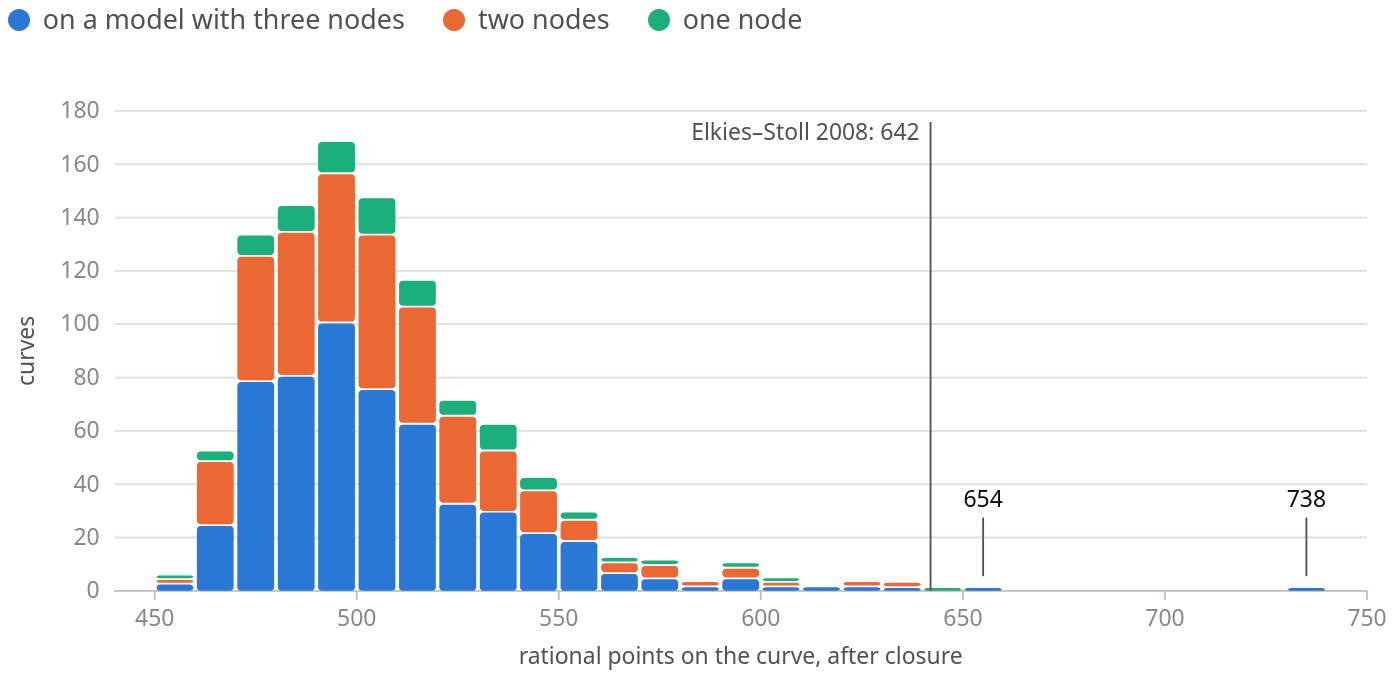
\includegraphics[width=0.9\linewidth]{figs/results.png}
\caption{The $1035$ different curves closed by the search, by number of rational points and by the number of nodes of the model.  Curves with fewer than $440$ points of height at most $10^5$ were not closed, so the left part of the picture is incomplete.}
\label{fig:results}
\end{figure}

Sixteen curves have at least $600$ points (Table~\ref{tab:top}), and three have at least $642$: $C_{738}$, the curve $C_{642}$
of Elkies and Stoll, which the search finds on the line $(95,-9,-82)$ of a one-node model with $106$ forced points, and
\begin{align*}
C_{654}\colon\quad y^2={}&963396x^6-25653180x^5-257315387x^4\\
&+5817403620x^3+43135861216x^2-76150919040x+48962544400 .
\end{align*}
It is the section by the line $(83,6,125)$ of a three-node model with $84$ forced points ($26$ tritangents and $16$ node
lines).  It has $570$ points of height at most $10^5$ and the closure adds $42$ $x$-values, for $654$ points.  Its Jacobian
is absolutely simple of rank at least $22$, its automorphism group has order $2$, and the Galois
group of the sextic is $S_6$.  On its model no other line has as many as $440$ points of height at most $10^5$, so this curve too
is an outlier line on an ordinary model.

\begin{table}[h]
\centering
\begin{tabular}{rrcrlcrr}
\toprule
points & of height $\le10^5$ & nodes & forced & model & line & score & rank\\
\midrule
$738$ & $662$ & $3$ & $78$ & \texttt{t0453} & $(66,\,31,\,-52)$ & $112$ & $1$\\
$654$ & $570$ & $3$ & $84$ & \texttt{t1272} & $(83,\,6,\,125)$ & $82$ & $1$\\
$642$ & $554$ & $1$ & $106$ & \texttt{b4} & $(95,\,-9,\,-82)$ & $80$ & $32$\\
$638^{*}$ & $604$ & $2$ & $92$ & \texttt{p144} & $(145,\,2,\,50)$ & $90$ & $1$\\
$636$ & $562$ & $2$ & $92$ & \texttt{p008} & $(154,\,-369,\,102)$ & $51$ & $629$\\
$632$ & $546$ & $3$ & $82$ & \texttt{t2139} & $(22,\,-295,\,-100)$ & $58$ & $49$\\
$626$ & $528$ & $2$ & $90$ & \texttt{p098} & $(225,\,219,\,112)$ & $47$ & $1067$\\
$620$ & $558$ & $3$ & $78$ & \texttt{t1782} & $(387,\,99,\,-16)$ & $46$ & $830$\\
$620$ & $544$ & $2$ & $94$ & \texttt{p101} & $(165,\,157,\,-106)$ & $76$ & $28$\\
$620$ & $538$ & $3$ & $78$ & \texttt{t0497} & $(291,\,130,\,-215)$ & $70$ & $33$\\
$614$ & $524$ & $3$ & $80$ & \texttt{t1614} & $(227,\,224,\,186)$ & $59$ & $110$\\
$610$ & $574$ & $3$ & $78$ & \texttt{t0555} & $(30,\,114,\,313)$ & $77$ & $7$\\
$604$ & $524$ & $3$ & $76$ & \texttt{t1068} & $(35,\,76,\,224)$ & $84$ & $4$\\
$604$ & $522$ & $3$ & $78$ & \texttt{t2005} & $(13,\,-230,\,1)$ & $64$ & $45$\\
$602$ & $552$ & $2$ & $92$ & \texttt{p053} & $(173,\,109,\,-56)$ & $80$ & $4$\\
$602$ & $512$ & $1$ & $108$ & \texttt{b5} & $(106,\,-113,\,-28)$ & $65$ & $242$\\
\bottomrule
\end{tabular}
\caption{The curves with at least $600$ rational points found by the search.  The model is the name of its row in
\texttt{data/models.txt}, and the line is given in the coordinates of that row.  The last two columns are the score of the line and
its position among the lines of its model ordered by score.  The
Jacobian of the curve marked $^*$ is isogenous to a product of two elliptic curves; the other fifteen are absolutely simple.}
\label{tab:top}
\end{table}

\emph{The curves are generic.}  For $1060$ of the $1061$ curves the sextic has Galois group $S_6$, so by Zarhin's
theorem~\cite{Zarhin} the Jacobian has endomorphism ring $\Z$ over $\overline\Q$: it is absolutely simple, and the curve has no
automorphism besides the hyperelliptic involution.  The exception is the curve with $638$ points in Table~\ref{tab:top}.  It
has an extra involution and its Jacobian splits, so it belongs with the curves of Keller--Kulesz type of the introduction, and it
has fewer points than the $648$-point curve.  (Curves with split Jacobian are a different subject with their own constructions;
they are not considered further here.)

\emph{Forced points do not predict the best curves.}  Between strata the number of forced points matters, as the table above
shows.  Within a stratum it does not help: among the three-node models the mean number of curves with at least $400$ points of
height at most $10^5$ \emph{falls} from $2.4$ per model for the models with $72$ forced points to $1.3$ for those with $84$ and
$0.8$ for the five with $86$ (rank correlation $-0.13$ over the $2188$ models; Figure~\ref{fig:forced}).  The models of the two
best curves have $78$ and $84$ forced points, of a possible $72$ to $86$, and on each of them no other line has as many as
$440$ points of height at most $10^5$.  The records are isolated lines on models that are otherwise unremarkable.

\begin{figure}[ht]
\centering
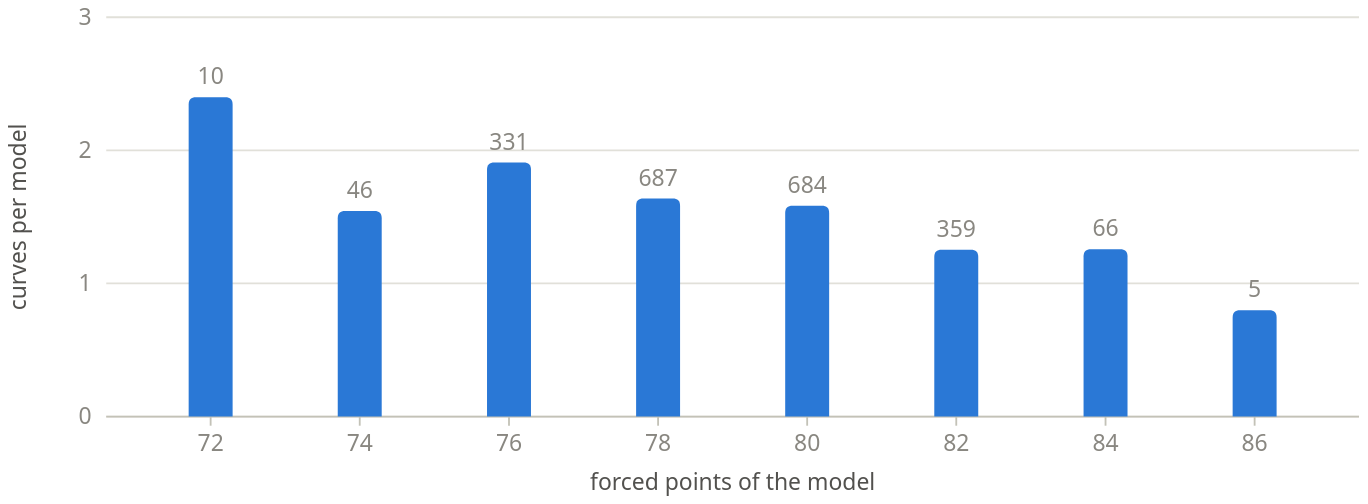
\includegraphics[width=0.9\linewidth]{figs/forced.png}
\caption{Three-node models: the mean number of curves with at least $400$ points of height at most $10^5$ on a model, by its number of forced points.  The number of models is written above each bar.}
\label{fig:forced}
\end{figure}

\subsection*{What the search does not cover}
\begin{itemize}\itemsep 1pt
\item \emph{Lines of height above $400$, and other coordinates.}  The bound is a choice of cost.  The height of a line is not a
natural limit, and it depends on the coordinates: a model can have several minimal sextics, and the search uses the one that the
construction happens to produce (Section~\ref{sec:models}).  An example is the model \texttt{b5}.  Its line $(327,-285,-512)$ cuts
out a curve with $614$ points, which the search does not see; on the other minimal sextic of that model given in
Section~\ref{sec:models} the same line is $(21,-256,-50)$.  We know nine further curves with at least $600$ points on these
models that the search does not find; they come from searches of particular models with larger bounds for the height, and are
not part of this computation.
\item \emph{Other models.}  The four three-node classes without a sextic, the models with a cusp, and all models with four or
more singular points, of which the census records tens of thousands.
\item \emph{Lines through a singular point}, whose curves have genus at most $1$.
\item \emph{Lines with a low score, and curves with low counts.}  A curve with many points is lost if the score of its line is
below $40$, or if it has fewer than $250$ points of height at most $2000$ or fewer than $330$ of height at most $10^4$.  For the
sixteen curves of Table~\ref{tab:top} the margins are comfortable: their scores are at least $46$, and they have at least $310$
points of height at most $2000$ and $400$ of height at most $10^4$.  For weaker curves they are not.  The curves closed do not
thin out towards the bound: seven of them have score $40$ and ten have score $41$, one of the former with $584$ points.
In a sample of $87$ models (all seven with one node, $20$ with two and $60$ with three) that were searched again with the bound
lowered to $30$ and the thresholds to $200$ and $300$, $152$ curves are closed, where the search above closes $144$ on the same
models.  The eight additional curves all have scores between $30$ and $39$: they are lost by the score bound, and none by the
thresholds.  Seven of them are on one-node models, and they have between $494$ and $556$ points.  So the search loses about one in
twenty of the curves that these lower settings would find; nothing in the sample suggests that it loses curves with $600$ points,
but a sample of this size cannot exclude it.
\item \emph{Curves that were not closed.}  The closure added between $6$ and $116$ points to a curve (median $42$).  The sixteen
curves with at least $600$ points have at least $512$ points of height at most $10^5$, well above the threshold of $440$, so a
curve below the threshold with $600$ points would need a larger gain than any we saw.  For smaller numbers the list is not
complete: curves with $550$ points appear with as few as $444$ points of height at most $10^5$.
\end{itemize}

\subsection*{Two remarks}
The first is that the number of forced points, which is what one sees first in a model, is a poor guide to its best curve.  The best
curves are isolated lines, and they turned up in the stratum with the fewest forced points of the three, because that stratum has
the most models.  The second is that the space of models is very large and almost entirely unexplored.  The strata with four or
more singular points contain tens of thousands of classes at least, none of which is searched here, and on the models that are
searched only the lines of height at most $400$ in one system of coordinates have been looked at.  There is no reason to think
that $738$ is the largest number of points on a line section of $\X_{163}$.

\section{Reproducing the results}\label{sec:files}

The programs, the data and the certificates are in the repository~\cite{Repo},
\url{https://github.com/AndrewVSutherland2/g2ratpoints738}.  They contain what is needed to check each statement, and to repeat
the computation from Elkies' sextic.  The file \texttt{README.md} of the repository says which file proves which statement,
what the programs need and how to run them.

\subsection*{Computations}
The programs that list surface points, score lines, count points and close them are C programs written for this project.  They use
AVX-512 instructions where the processor has them (the two sieves treat $512$ values at a time) and plain C otherwise: the output
is the same, and the search then takes about twice as long.  The lattice computations and the construction of the models use
PARI/GP~\cite{PARI} (2.18.1) and Magma~\cite{Magma} (V2.29-10), and the certificates use Magma.  Everything ran under Linux on one
machine with a $16$-core AMD Ryzen AI Max+ 395 processor (Zen~5, up to $5.2$\,GHz, $32$ threads).

The whole computation, from Elkies' sextic to the curves, took $62$ minutes on that machine:
\begin{center}\small
\begin{tabular}{lrr}
\toprule
part & minutes & processor hours\\
\midrule
constructing the models & $7.3$ & $3.5$\\
listing the points of the surfaces & $27.5$ & $13.4$\\
scoring the lines & $5.1$ & $2.3$\\
the curves of the lines kept & $21.9$ & $9.6$\\
\quad restriction and reduction & $3.2$ & $1.4$\\
\quad points of height at most $2000$ & $7.6$ & $3.4$\\
\quad points of height at most $10^4$ & $1.6$ & $0.6$\\
\quad points of height at most $10^5$ & $7.7$ & $3.4$\\
\quad closure & $1.7$ & $0.7$\\
\midrule
total & $61.8$ & $28.8$\\
\bottomrule
\end{tabular}
\end{center}
Sixteen models are searched at a time, on two threads each, so the parts of the search overlap; its time is divided among them
in proportion to the time that the sixteen jobs spent in each.

The only statement of this note that depends on an unproved hypothesis is the upper bound for the rank, where Magma's class group
computations assume GRH.  Canonical heights are computed numerically; they enter only the regulator and the enumeration of
Section~\ref{sec:curve}, which is evidence and not a proof.

\section*{AI use}
The search, the computations, and the text and figures of this note were produced by Claude Fable 5.2 (Anthropic), working under
the direction of the author, who posed the problem and supervised the work.  ``We'' refers to both.

\section*{Acknowledgments}
We thank GPT-6 Astra (OpenAI) for helpful reviews of two earlier drafts of this manuscript.

\begin{thebibliography}{99}\small\itemsep 0pt
\bibitem{BruinStoll} N.~Bruin, M.~Stoll, \emph{The Mordell--Weil sieve: proving non-existence of rational points on curves}, LMS J.\ Comput.\ Math.\ \textbf{13} (2010), 272--306, \href{https://doi.org/10.1112/S1461157009000187}{doi:10.1112/S1461157009000187}.
\bibitem{CHM} L.~Caporaso, J.~Harris, B.~Mazur, \emph{Uniformity of rational points}, J.~Amer.\ Math.\ Soc.\ \textbf{10} (1997), 1--35, \href{https://doi.org/10.1090/S0894-0347-97-00195-1}{doi:10.1090/S0894-0347-97-00195-1}.
\bibitem{Degtyarev} A.~Degtyarev, \emph{Smooth models of singular K3-surfaces}, Rev.\ Mat.\ Iberoam.\ \textbf{35} (2019), 125--172, \href{https://doi.org/10.4171/rmi/1051}{doi:10.4171/rmi/1051}.
\bibitem{ElkiesClay} N.~D.~Elkies, \emph{About the cover: Rational curves on a K3 surface}, in: Arithmetic Geometry, Clay Math.\ Proc.\ \textbf{8}, Amer.\ Math.\ Soc., 2009, 1--4.
\bibitem{ElkiesSI} N.~D.~Elkies, \emph{Mordell--Weil generators for singular Shioda--Inose surfaces over $\Q$}, web page, \url{https://people.math.harvard.edu/~elkies/K3_20SI.html} (accessed 17 November 2026).
\bibitem{ElsenhansStoll} A.-S.~Elsenhans, M.~Stoll, \emph{Minimization of hypersurfaces}, Math.\ Comp.\ \textbf{93} (2024), 2513--2555, \href{https://doi.org/10.1090/mcom/3924}{doi:10.1090/mcom/3924}, \href{https://arxiv.org/abs/2110.04625}{arXiv:2110.04625}.
\bibitem{Epoch} Epoch AI, \emph{Many rational points on a genus-2 curve}, FrontierMath: Open Problems, \url{https://epoch.ai/frontiermath/open-problems/genus-2-rational-points} (accessed 14 November 2026).
\bibitem{Inose} H.~Inose, \emph{Defining equations of singular K3 surfaces and a notion of isogeny}, in: Proceedings of the International Symposium on Algebraic Geometry (Kyoto, 1977), Kinokuniya, Tokyo, 1978, 495--502.
\bibitem{KK} W.~Keller, L.~Kulesz, \emph{Courbes alg\'ebriques de genre $2$ et $3$ poss\'edant de nombreux points rationnels}, C.~R.\ Acad.\ Sci.\ Paris S\'er.~I Math.\ \textbf{321} (1995), 1469--1472.
\bibitem{Magma} W.~Bosma, J.~Cannon, C.~Playoust, \emph{The Magma algebra system I: The user language}, J.~Symbolic Comput.\ \textbf{24} (1997), 235--265, \href{https://doi.org/10.1006/jsco.1996.0125}{doi:10.1006/jsco.1996.0125}.
\bibitem{MuellerStoll} J.~S.~M\"uller, M.~Stoll, \emph{Canonical heights on genus-2 Jacobians}, Algebra Number Theory \textbf{10} (2016), 2153--2234, \href{https://doi.org/10.2140/ant.2016.10.2153}{doi:10.2140/ant.2016.10.2153}.
\bibitem{Nikulin} V.~V.~Nikulin, \emph{Integral symmetric bilinear forms and some of their applications}, Math.\ USSR Izv.\ \textbf{14} (1980), 103--167, \href{https://doi.org/10.1070/IM1980v014n01ABEH001060}{doi:10.1070/IM1980v014n01ABEH001060}.
\bibitem{PARI} The PARI~Group, \emph{PARI/GP version 2.18.1}, Univ.\ Bordeaux, \url{https://pari.math.u-bordeaux.fr/}.
\bibitem{SaintDonat} B.~Saint-Donat, \emph{Projective models of K-3 surfaces}, Amer.\ J.\ Math.\ \textbf{96} (1974), 602--639, \href{https://doi.org/10.2307/2373709}{doi:10.2307/2373709}.
\bibitem{ShiodaSandwich} T.~Shioda, \emph{Kummer sandwich theorem of certain elliptic K3 surfaces}, Proc.\ Japan Acad.\ Ser.~A Math.\ Sci.\ \textbf{82} (2006), 137--140, \href{https://doi.org/10.3792/pjaa.82.137}{doi:10.3792/pjaa.82.137}.
\bibitem{ShiodaInose} T.~Shioda, H.~Inose, \emph{On singular K3 surfaces}, in: Complex Analysis and Algebraic Geometry, Iwanami Shoten, Tokyo, 1977, 119--136, \href{https://doi.org/10.1017/CBO9780511569197.010}{doi:10.1017/CBO9780511569197.010}.
\bibitem{Stoll2desc} M.~Stoll, \emph{Implementing $2$-descent for Jacobians of hyperelliptic curves}, Acta Arith.\ \textbf{98} (2001), 245--277, \href{https://doi.org/10.4064/aa98-3-4}{doi:10.4064/aa98-3-4}.
\bibitem{ratpoints} M.~Stoll, \emph{Documentation for the \texttt{ratpoints} program}, \href{https://arxiv.org/abs/0803.3165}{arXiv:0803.3165}.
\bibitem{StollAvg} M.~Stoll, \emph{On the average number of rational points on curves of genus $2$}, \href{https://arxiv.org/abs/0902.4165}{arXiv:0902.4165}.
\bibitem{StollExp} M.~Stoll, \emph{Rational points on curves of genus $2$: experiments and speculations}, Dagstuhl Seminar Proceedings 09221 (2009), \href{https://doi.org/10.4230/DagSemProc.09221.5}{doi:10.4230/DagSemProc.09221.5}.
\bibitem{StollRecord} M.~Stoll, \emph{A genus $2$ curve with at least $642$ rational points}, web page, \url{https://mathe2.uni-bayreuth.de/stoll/recordcurve.html}.
\bibitem{Repo} A.~V.~Sutherland, \emph{A genus $2$ curve with $738$ rational points: the computation}, GitHub repository \texttt{g2ratpoints738}, 2026, \url{https://github.com/AndrewVSutherland2/g2ratpoints738}.
\bibitem{Voight} J.~Voight, \emph{Kneser's method of neighbors}, \href{https://arxiv.org/abs/2308.11566}{arXiv:2308.11566}.
\bibitem{Zarhin} Yu.~G.~Zarhin, \emph{Hyperelliptic Jacobians without complex multiplication}, Math.\ Res.\ Lett.\ \textbf{7} (2000), 123--132, \href{https://doi.org/10.4310/MRL.2000.v7.n1.a11}{doi:10.4310/MRL.2000.v7.n1.a11}.
\end{thebibliography}

\appendix
\section{The map between the two models}\label{app:map}
The lifts of the conics $q_1,q_2$ of Section~\ref{sec:models} are given by the cubic forms
{\small
\begin{align*}
G_1&=120x_0^3-\bigl(\tfrac{4090}{9}x_1+158x_2\bigr)x_0^2+(-2305x_1^2+39x_1x_2)x_0-2280x_1^3+\tfrac{2056}{9}x_1^2x_2,\\
G_2&=-1920x_0^3+(4480x_1+624x_2)x_0^2+\bigl(-\tfrac{20887}{9}x_1^2+666x_1x_2+9x_2^2\bigr)x_0-\tfrac{1463}{9}x_1^3-\tfrac{38}{9}x_1^2x_2+9x_1x_2^2 .
\end{align*}}
in the sense that $S_E\equiv G_i^2$ modulo $q_i$ and $\Gamma_i=\{q_i=0,\ w=G_i\}$.  The coordinate functions of the new model are
$z_i=A_i+B_iw$ with
\[
B_0=-800x_0+1980x_1-260x_2,\quad B_1=8800x_0-15130x_1+350x_2,\quad B_2=-3325x_1+1255x_2,
\]
{\small
\begin{align*}
A_0={}&1536000x_0^4-(3801600x_1+1198080x_2)x_0^3+(-1812000x_1^2+1139328x_1x_2+2208x_2^2)x_0^2\\
&+(4484700x_1^3+2145348x_1^2x_2-204876x_1x_2^2+3276x_2^3)x_0\\
&+704484x_1^3x_2-42516x_1^2x_2^2-2004x_1x_2^3+36x_2^4,\\
A_1={}&22272000x_0^4+(-47331200x_1+504960x_2)x_0^3+(-6552400x_1^2+3901184x_1x_2-73776x_2^2)x_0^2\\
&+(30724050x_1^3-4682002x_1^2x_2+298950x_1x_2^2-3798x_2^3)x_0\\
&+2257200x_1^4-393572x_1^3x_2-53660x_1^2x_2^2+3156x_1x_2^3-36x_2^4,\\
A_2={}&19584000x_0^4+(-31806400x_1+594240x_2)x_0^3+(-13242200x_1^2+276256x_1x_2-241224x_2^2)x_0^2\\
&+(24965625x_1^3-2984177x_1^2x_2+59235x_1x_2^2-243x_2^3)x_0\\
&+1128600x_1^4+1038206x_1^3x_2-143086x_1^2x_2^2+7770x_1x_2^3-18x_2^4 .
\end{align*}}

\section{A Magma certificate for the model}\label{app:magma}
The following script, \texttt{k3model.m}, proves the statements about the model of $C_{738}$ made in Section~\ref{sec:models} from
the sextic $S_3$ and its $39$ lines alone.  It runs in a few seconds.
{\fontsize{7}{8.6}\selectfont\verbatiminput{k3model.m}}
\end{document}
